\documentclass[a4paper,11pt,column]{article}
\usepackage[latin1]{inputenc}
\usepackage[english]{babel}
\usepackage{amsmath}
\usepackage{amsfonts}
\usepackage{amssymb}
\usepackage{wasysym}
\usepackage{cuted}
\usepackage{pdfpages}

\usepackage{titling}
\usepackage{siunitx}
\usepackage[style=ieee,backend=bibtex]{biblatex}
\addbibresource{designbib.bib}
\usepackage[font={small}]{caption}
\usepackage{subfig}
\usepackage{nomencl}

\usepackage{graphicx}
\usepackage{color}

\usepackage{booktabs}
\usepackage{threeparttable}
\usepackage{fancyhdr}
\usepackage{float}

\usepackage{varioref}
\usepackage{textcomp}
\usepackage{xspace}
\usepackage[activate={true,nocompatibility},final,tracking=true,kerning=true,spacing=nonfrench,factor=1100,stretch=10,shrink=10]{microtype}

% Top matter.
\author{Group 25}
\title{Design Report}
\date{\today}

% Header and footer.
\pagestyle{fancy}
\fancyhf{}
\lhead{\thetitle}
\rhead{\theauthor}
\cfoot{\thepage}
\renewcommand{\headrulewidth}{0pt}
\renewcommand{\footrulewidth}{0pt}

\begin{document}

%% Title page.
\begin{titlepage}
    \centering
    \vspace*{\fill}
    
\includegraphics[width=\textwidth]{Images/Durham.jpg}
    \vspace*{\fill}
    \LARGE\thetitle\\
    \large\theauthor\\
    \large P.H. Gaskell, K. Blundy\\
    \large L2 Design\\
    \large\thedate\\
    \vspace*{\fill}
\end{titlepage}

\section{Executive Summary}

Microphonic effects exist in Hi-Fi systems wherein mechanical vibrations are 
transformed into unwanted electrical signals, termed noise, that consequently 
reduce sound quality. Isofonics have designed footers of aluminium and steel 
upon which such systems are to be supported that aim to isolate and attenuate 
the signals responsible for this aforementioned noise. Three footers are 
required per system, three being the minimum number of points of contact 
necessary to support a rigid mass, and are to be sold as a device comprising a 
contained magnetic damping mechanism with two optional additional pieces: a 
removable base to use the device as a stand alone mount as opposed to its 
mounting within existing equipment and a removable spike offering a minimal 
point of contact. The main device, base and spike are to cost \textsterling 
blah, \textsterling blah and \textsterling blah respectively, placing Isofonics 
at the higher end of the existing market due to its premium quality components 
embodying a design that is both innovative and effective. The device may be 
altered manually by the user to support a range of different masses, a feature 
of customisability unique to Isofonics. This process may also be informed by a 
user friendly phone application. Additionally, within this design lies 
potential for product families of differing size, catering to an even wider 
audience, and applications within the field of optics, more specifically in the 
optimisation of microscopes.

% Nomenclature.
\makenomenclature

% Acronyms
\nomenclature[A0]{CNC}{Computer Numerical Control}
\nomenclature[A1]{DFA}{Design for Assembly}
\nomenclature[A2]{DFM}{Design for Manufacture}
\nomenclature[A3]{EMF}{Electromotive Force}
\nomenclature[A4]{URS}{User Requirement Specification}

% Variables

\printnomenclature

% Table of contents.
\tableofcontents

% Main matter.
\section{Introduction}
Microphonics describes the phenomenon wherein internal components within an 
electronic device transform mechanical vibrations into undesired electrical 
signals\cite{microphonics}. In the context of hi-fi systems, and when these 
vibrations are within the frequency range audible to the human 
ear---20~Hz--20~kHz---they equate to noise that reduces audio quality and 
therefore 
threatens 
the user\textquotesingle s listening experience. This report details the design 
of vibration isolation and attenuation mounts that minimise this interference 
as well as that originating from external sources. 

The following function analysis tree defines the user requirement specification 
for the product:

\begin{figure}[h]
   \centering
   \includegraphics[width=\textwidth]{Images/URSTree}
   \caption{User Requirement Specification Diagram}
   \label{}
\end{figure}

With such a niche product consisting of high tolerance machined parts and 
premium materials comes a high cost, indicating a corresponding market; middle 
aged/mature clientele with strong technical understanding of the hobby and its 
principles or affluent younger hobbyists. The current market offers a range of 
mounts at a range of prices within which our product shall lie at the higher 
end, namely between \textcolor{red}{\textsterling 1500--\textsterling 2000} 
per mount. 

Market leaders such as Stillpoints\textsuperscript{\textregistered}, 
Nordost\textsuperscript{\textregistered} and 
Isoclear\textsuperscript{\textregistered} offer sleek solutions yet lack the 
tailorability offered by our design, allowing customers to pre-load their 
mounts manually for individual amps, potentially with interactivity provided by 
an instructive technical app. After conducting market research via surveys, it 
was found that potential customers were very much interested in the ability to 
manually adjust their mount as appropriate and that this offered an invaluable, 
unique selling point.

This report covers the initial design concepts proposed by Group 25, the 
development of a chosen design, its design for manufacture and sustainability 
and its commercial considerations.

\section{Design Concepts}

During initial research it was noticed the most successful products on the 
market met three primary criteria:

\begin{itemize}
    \item They allowed the mounted equipment to move with four degrees of 
    freedom: three in translation and one in rotation.
    \item They used single degree of freedom systems for damping. Simpler 
    damping mechanisms were more effective at consistently attenuating 
    unwanted frequency components.
    \item Vibrations were efficiently transmitted to the damping system from 
    the equipment. This was typically achieved using hard materials and limited 
    contact between the footer and equipment.
\end{itemize}

In summary, any concepts generated had to first \emph{isolate} the equipment 
then \emph{attenuate} vibrations by allowing the equipment to move freely and 
then damp vibrations in controlled manner.

In order to simplify the process of concept generation, the formulation of 
isolation and attenuation mechanisms was separated. Isolation mechanisms were 
designed to translate the four degrees of freedom in the movement of the 
equipment into the single degree of freedom of the damping mechanism. Those 
single degree of freedom damping mechanisms were designed to be easily applied 
to multiple isolation concepts.

\subsection{Damping Mechanisms} \label{sec:damping_mechanisms}

Three methods of damping were considered---not including the friction in 
bearings, which cannot be completely eliminated. These were viscoelastic, 
magnetic and fluid damping.

Viscoelastic materials, such as rubber or Sorbothane\textregistered, heat up 
when subjected to changes in mechanical stress \cite{meyers2009mechanical}. 
Hence, the amplitude of vibrations are reduced when the driving oscillations 
are transmitted through viscoelastic materials. Typically when these materials 
are used in footers, the vibrations are not limited to a single degree of 
freedom, so the effectiveness of attenuation depends on the vibration 
direction. This makes it difficult to model and specify a single system natural 
frequency or damping factor.

Figure~\vref{fig:viscoelastic} details how viscoelastic materials can be used 
in a system where vibrations have been translated to a single direction. A 
linear bearing compresses a viscoelastic sleeve on the same shaft.

\begin{figure}[h] 
    \centering
    \textbf{VISCOELASTIC DAMPING CONCEPT}
    \caption{D1---Viscoelastic damping mechanism.}
    \label{fig:viscoelastic}
\end{figure}

Magnets can also be used to damp vibrations when constrained to a single 
direction. As a permanent magnet travels through a coil, an EMF is induced due 
to Faraday's law, which drives a current when the circuit is complete. The 
current flowing generates a magnetic field opposing the permanent magnet, 
according to Lenz's law. A possible assembly for this system is detailed in 
Figure~\vref{fig:magnetic}. The strength of magnets were to be tuned to the 
desired dynamic properties of the system.

\begin{figure}[h] 
    \centering
    \textbf{MAGNETIC DAMPING CONCEPT}
    \caption{D2---Magnetic damping mechanism.}
    \label{fig:magnetic}
\end{figure}

Finally, a simple fluid damping system was considered, whereupon a bearing 
travels through some viscous fluid. Skin friction provides the damping force in 
Figure~\vref{fig:fluidic}. The size of the bearing could be tuned to meet the 
required constraints for damping factor and natural frequency. However, this 
concept was difficult to realise in any manufacturable assembly whilst 
successfully containing the fluid.

\begin{figure}[h] 
    \centering
    \textbf{FLUIDIC DAMPING CONCEPT}
    \caption{D3---Fluidic damping mechanism.}
    \label{fig:fluidic}
\end{figure}

\subsection{Isolation Mechanisms}

Early concepts made use of linkages to transform vertical and lateral 
oscillations into lateral oscillations along damped linear bearings, which 
would have been most easily realised using a viscoelastic damper. 
Figure~\vref{fig:concept1} details one such embodiment.

\begin{figure}[h] 
    \centering
    \textbf{ELOISE'S LINKAGE CONCEPT}
    \caption{C1---Simple linkage mechanism.}
    \label{fig:concept1}
\end{figure}

Some components of vertical vibrations were not damped by the mechanism in 
Figure~\ref{fig:concept1}; these were transmitted to the base of the mount such 
that the mount was not completely isolated. Repeating the mechanism by using 
multiple layers of linkages was explored in the concept detailed in 
Figure~\vref{fig:concept2}. Each layer damps a fraction of the vertical 
oscillations transmitted downwards by the layer above resulting in more 
isolation.

\begin{figure}[h]
    \centering
    \textbf{RUSSELL'S LINKAGE CONCEPT}
    \caption{C2---Layered linkage mechanism.}
    \label{fig:concept2}
\end{figure}

However, the fundamental issue with linkage based isolaton mechanisms is the 
feature size of those linkages. Thin members are prone to resonance with large 
amplitudes at relatively lower frequencies \cite{citation needed}, possibly 
within the audible spectra (20 Hz--20 kHz).

Spherical bearings also featured in design concepts. Figure~\vref{fig:concept3}
describes one such embodiment where a layer of spherical bearings were
sandwiched between two platforms. The upper platform was to be made of a hard 
material such as stainless steel or tungsten carbide, in order to efficiently 
transmit vibrations through to the bearings via point contacts. The bearings 
allowed the top platform to move with the equipment in three degrees of 
freedom: two lateral directions and lateral rotation. The bottom platform would 
have been made of some viscoelastic material with holes for the bearings to 
rest in. Both vertical and lateral oscillations would have been damped by this 
platform and dissipated as heat.

This concept had a major drawback: the damping mechanism was not confined to a 
single degree of freedom. It would have been challenging to determine a single 
damping factor and resonant frequency. The isolation mechanism was an anomaly 
in the concept generation phase, as the damping mechanism was not 
interchangable with those in Section~\vref{sec:damping_mechanisms}.

\begin{figure}[h]
    \centering
    \textbf{GEORGE'S PLATFORM CONCEPT}
    \caption{C3---Viscoelastic platform concept.}
    \label{fig:concept3}
\end{figure}

Isolation cones are a popular type of mount, an example is Nordost's Sort 
Kones\textregistered. The Sort Kones are made of three parts: a post, spherical 
bearing, and cone. The bearing rests on the top of the post and the cone sits 
on top of the bearing, such that the cone is free to swivel and rotate. 
However, cones seek only to isolate the mounted equipment and allow free 
movement---they do not attenuate vibrations.

Figure~\vref{fig:concept4} demonstrates how an attenuating mechanism could have 
been incorporated into the post of an isolation cone. The spring in the 
isolation mechanism could have been replaced with one of the damping mechanisms 
in Figure~\ref{fig:viscoelastic} and Figure~\ref{fig:magnetic}.


\begin{figure}[h]
    \centering
    \textbf{MAT'S CONE CONCEPT}
    \caption{C4---Damped cone concept.}
    \label{fig:concept4}
\end{figure}

An alternative mechanism was devised to translate horizontal and lateral 
oscillations into oscillations of a spherical bearing along a race. 
Figure~\vref{fig:concept5} details the geometry required to achieve this 
translation.

\begin{figure}[h]
    \centering
    \textbf{RUSSELL'S POINTY BOTTOM CONCEPT}
    \caption{C5---Cone and bearing concept.}
    \label{fig:concept5}
\end{figure}

When no force is applied to the top piece, the bearing would travel to the 
bottom of its race. Increasing the load would cause the bearing to move up the 
race due to the gradient of the curve on the top piece, which was greater than 
the gradient of the race. There would be some component of the reaction force 
acting on the bearing perpendicular to the curve which points up the the slope 
of the race. However, the gradient of the curve decreases travelling up the 
slope, so for a given load the component of the reaction force would also 
decrease. Therefore, for each load, there is a different equilibrium position 
somewhere along that race where the components of the bearing's weight and the 
reaction force acting on the bearing in the direction of the race are equal and 
opposite. The mechanism acts as a geometric spring with some stiffness.

The frictional sheer forces in the mechanism would provide significant damping 
due to the magnitude of the reaction forces involved. Furthermore, one of the 
damping mechanisms in Figure~\ref{fig:viscoelastic} or 
Figure~\ref{fig:magnetic} could be coupled to the linear motion of the 
bearings to tune the system to a desired natural frequency and damping 
factor---this could result in quite a large footer.

A drawback of this concept is difficulty in containing the bearings, the user 
would be free to remove the top piece, and the bearings would all come out of 
their races. Competitors could easily see how the mechanism works and replicate 
it for themselves.

Figure~\vref{fig:concept6} details a variation of C5, whereby the bearings 
travel outwards up the slope. This creates more space for a damping mechanism 
for each race around the outside of the footer. A fluid could be contained in 
the cavity in the bottom piece to damp vibrations using the mechanism described 
in Figure~\ref{fig:fluidic}.

\begin{figure}[h]
    \centering
    \textbf{RUSSELL'S POINTY TOP CONCEPT}
    \caption{C6---Alternative cone and bearing concept.}
    \label{fig:concept6}
\end{figure}

The flexibility of the alternative cone and bearing concept C6, coupled with 
its innovative design set the concept apart from its alternatives. In 
\cite{maguire2016vibration}, it was shown how concept C6 with damping mechanism 
D2 best matched the customer's expectations and engineering requirements. This 
is the concept which informed the next stage of development and our final 
design.

\section{Design Development}

Through an iterative process, the concept highlighted in 
\cite{maguire2016vibration} for its promise was increasingly refined to produce 
a final design. The key milestones in development are as follows:

\begin{itemize}
    \item The transition from curved geometry to opposing pairs of rare earth 
    magnets to support the load of equipment.
    \item The addition of a user-adjustable preloading mechanism to increase 
    the range of masses that could be supported to full mass range of 
    amplifiers: 5~\si{\kilogram}--30~\si{\kilogram}~\cite{citation needed}.
    \item The casing required to contain the isolation mechanism were     
    considered.
\end{itemize}

\subsection{Opposing Magnets}
\subsubsection{Magnet Simulation}

As the footer houses 12 rare earth magnets, considerations have to be made for 
the way in which these magnets interact with the surroundings of the footer as 
they could cause damage or interfere with mounted or surrounding 
equipment footer. Using a software package called 
MagNet\textsuperscript{\textregistered} produced by 
infolytica\textsuperscript{\textregistered}, it was possible to perform a 2D 
finite element analysis of the footers, allowing the effects of these magnets 
to be modelled. The analysis performed in this section is for the geometry of 
the final design, but the same procedure was performed following each 
significant revision during the design process. When modelling the effect of 
these magnets the two extreme cases were considered: at minimum and maximum 
separation as detailed in Figure~\ref{figure:minsep} and 
Figure~\ref{figure:maxsep}.

\begin{figure}[h]
    \centering
    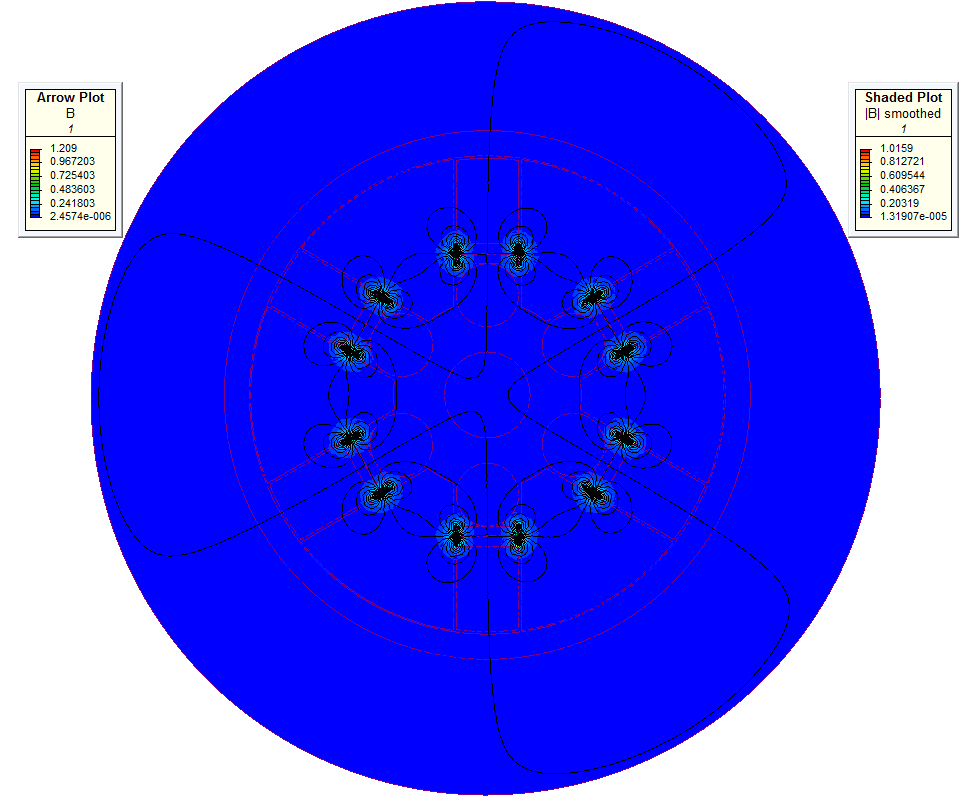
\includegraphics[width=\textwidth]{Images/maxpreload.png}
    \caption{Flux state with minimum separation of magnets}
    \label{figure:minsep}
\end{figure}

\begin{figure}[h]
    \centering
    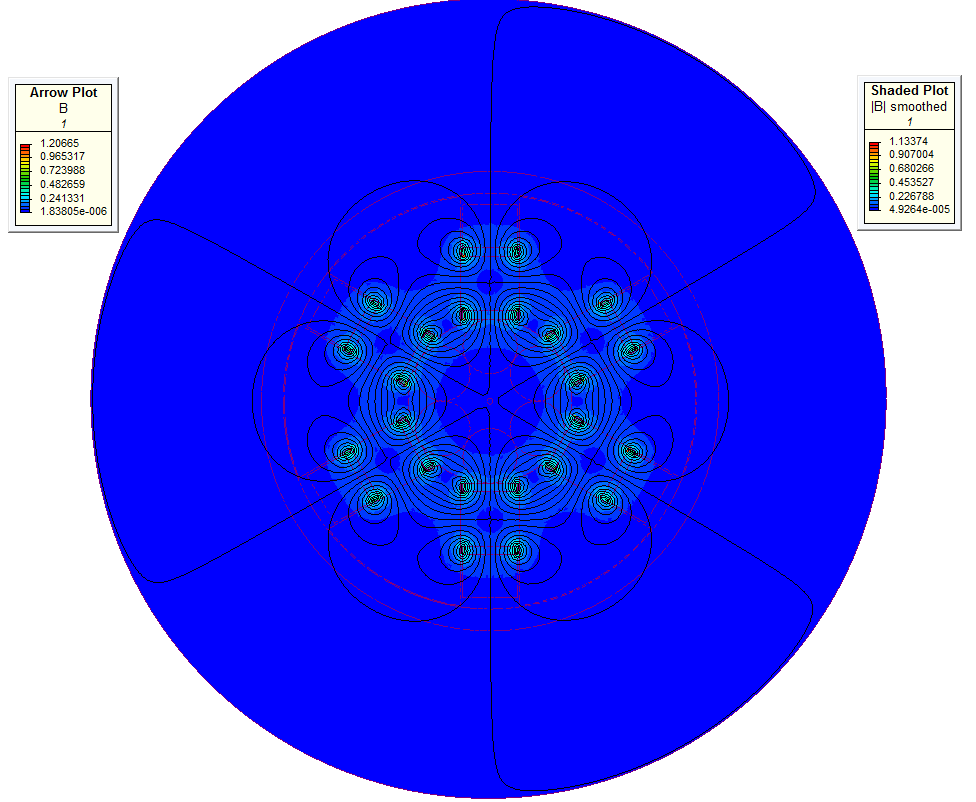
\includegraphics[width=\textwidth]{Images/minpreload.png}
    \caption{Flux state with maximum separation of magnets}
    \label{figure:maxsep}
\end{figure}

It can be seen that the flux density outside of the footer is negligible as it 
has a value of the order $10^{-5}$~\si{\tesla} meaning that there would be 
minimal to no interactions between the footer and its surroundings as nearly 
all of the magnetic flux is contained within the core of the device.

\subsection{Preloading Mechanisms}
\subsection{Casing}
\subsection{Materials}

\subsection{Materials}

Neodymium magnets are the most widely used type of rare-earth magnet, are the 
strongest type of permanent magnet commercially available and are of greatest 
benefit in applications where there is limited space. The magnetic properties 
termed remanence, coercivity and energy product dictate the performance of 
neodymium magnets. They measure the strength of the magnetic field, the 
material?s resistance to becoming demagnetized and the density of magnetic 
energy respectively. Given that there are numerous grades available, an 
overview of the range of values are outlined in Table 1. [1] The grade chosen 
for the project was N45SH, coated with three layers (nickel, copper and nickel) 
to reduce corrosion and provide a smooth finish. The brittleness of the magnets 
was also compensated for such that it does not undergo shear force during the 
cyclic loading. 

Tungsten carbide possesses Young?s modulus 530 GPa, more than two times of that 
for the grade of stainless steel chosen (190 ? 203 GPa) [4] [5]. Due to Hooke?s 
law, the material does not undergo large deflections which in turn ensured 
efficient energy transfer between the Hi-Fi components. The bearings do not 
require any lubrication as they grind down any particulates that may enter the 
system.

Steel is harder, and therefore more expensive, to machine than softer materials 
however, its properties make it invaluable to the quality of the product (see 
Section~\ref{sec:DetailDesign}) and pose no problem for the advanced machining 
capabilities of today. The product's entire composition out of steel was 
initially proposed but after receiving a quote from 'Sylatech' (r/c), a 
machining company in the northeast of England for �---- per piece, it was 
evident some optimisation was required to quote a retail price for our product 
that allowed for a 35\% \cite{ProfitMargins} profit margin.For this reason, it 
was decided that all non-critical parts may be machined from aircraft grade 
aluminium (6061-T6), an alternative roughly 1.5 times cheaper\cite{AluVSteel} 
than steel. 'Non-critical' in this context refers to all parts excluding the 
complex central piece (COR080-0003), the top piece (TOP080-0004) and removable 
spike (USR080-0001). For these parts, steel is required to contain magnetic 
flux leakage, remain unaffected by frictional effects of the moving bearings 
and not yield under concentrated stress. Additionally, aluminium is roughy 5 
times easier to machine than stainless steel\cite{AluVSteel} saving 
significantly on time, and therefore cost.

\subsubsection{Static Analysis}
\subsection{Dynamic Analysis}
\subsubsection{Parametric Model} \label{sec:parametric-model}
\subsubsection{System Tuning}
\subsubsection{Experimentation} \label{sec:experimentation}

To assess the effectiveness of the product, acceleration data from a vibrating 
amplifier was recorded to determine the frequency content of the signal to be 
attenuated. The same setup was used to capture acceleration data from the 
amplifier when mounted on half squash balls, which was later compared to the 
output of a dynamic model representing the final mount design using the 
undamped acceleration data captured as the model input. Squash balls were used 
to isolate Hi-Fi systems before footers entered the market and are an entry 
level alternative to footers.

A USB PicoScope\footnote{Pico Technology PicoScope 2204A} was used to capture 
the output of an accelerometer\footnote{STMicroelectronics LIS344ALH} at a 
sample rate of 50~\si{\kilo\hertz} for 10~\si{\second}. Human hearing ranges 
from 20~\si{\hertz}--20~\si{\kilo\hertz}; according to Nyquist, the sample rate 
had to be at least twice 20~\si{\kilo\hertz} to determine the power of these 
frequency components. 

The accelerometer was coupled to the top of an amplifier connected to a 
standard AC mains power supply---nominal voltage of 240~\si{\volt} at a 
frequency of 50~\si{\hertz}. Data from the accelerometer was captured for three 
conditions: with the amplifier turned off, on, and the amplifier turned on 
whilst sitting on half squash balls.

The data captured came in the form of a voltage output. To determine the 
acceleration from this information it was necessary to form a transfer
equation. To do so, the technical data sheet for the accelerometer 
\cite{SensorManual} was found and in it there was clear conversion which lead 
to the following
\begin{equation} \label{eq:acceleration}
    \ddot{y} = 9.81\cdot(0.66\cdot V - 1.65)
\end{equation}
where $a$ is the acceleration in \si{\meter\per\square\second} and $V$ is the 
voltage measured in \si{\volt}. Equation~\ref{eq:acceleration} is linear, so 
has no affect on the shape of the spectra. The spectra of the measured voltages 
were analysed instead.

Firstly, the data for the amplifier when off---the control---was compared to 
the amplifier when on; their spectra up to 1~\si{\kilo\hertz} are shown in 
Figure~\vref{fig:MatGraphs1}. There were no observable components above the 
noise floor in the range 1~\si{\kilo\hertz}--25~\si{\kilo\hertz}.

\begin{figure}[h]
    \centering
    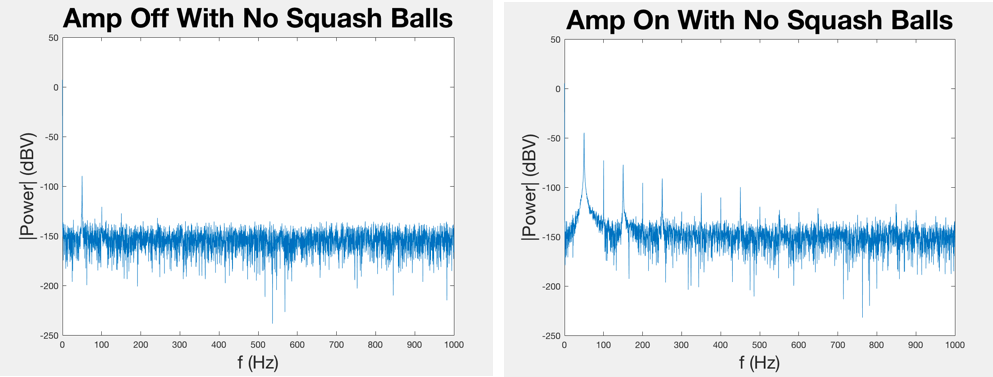
\includegraphics[width=\textwidth]{Images/MatGraphs}
    \caption{Compared Frequency Responses when Amplifier off and on}
    \label{fig:MatGraphs1}
\end{figure}

The spectra for amplifier when off had a fundamental at 50~\si{\hertz}. This is 
likely due to interference from other mains powered devices in the room---air 
conditioning, PCs and desktop power supplies for example. Contrasting this 
control spectra to the spectra for the amplifier when turned on, the 
fundamental frequency increased in power significantly from $-90$~\si{dBV} to 
$-40$~\si{dBV}---a factor of $10^5$. The harmonics can be seen at 
50~\si{\hertz} intervals although the noise floor due to the error of the 
accelerometer remained at $-140$~\si{dBV}.

Next, the spectra for the amplifier when on was compared to the spectra for the 
amplifier damped using squash balls. Figure~\vref{fig:MatGraphs2} reveals the 
effect the squash balls had on the frequency content of observed vibrations. 

The fundamental remains constant in frequency and power. However, from the 
simple damping the squash balls provide, the noise has been significantly 
cleared up, along with this success the harmonics have consistently lower 
peaks. This provides an example of successful damping which can be used as a 
comparison to the later mathematically damped data using dynamic model. The aim 
is to further clean up the noise and lower the power of the harmonics as much 
as possible, preferably below the noise floor which should lead to a reduction 
in microphonic effects and increase in sound quality.

\begin{figure}[h]
    \centering
    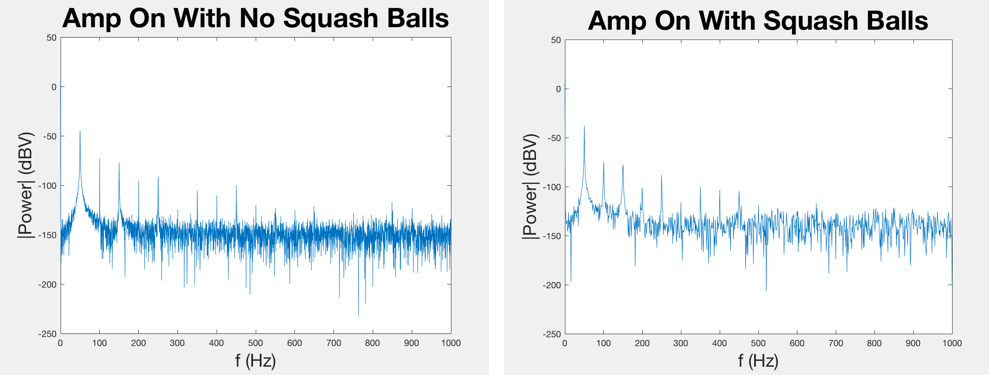
\includegraphics[width=\textwidth]{Images/MatGraphs2}
    \caption{Compared Frequency Responses with and without Squash Balls}
    \label{fig:MatGraphs2}
\end{figure}

\subsubsection{Dynamic Simulation}

It was determined that a dynamic model of the system would be necessary to 
quantify the potential success of the product. This could visually display the 
effects of the footers on attenuation of a signal from a Hi-Fi system, and 
hence inform whether the sound quality would be improved.

The three footers and mounted equipment can be simplified to a spring-mass 
damper system with non-linear stiffness---a driving force $F_d$ is supplied by 
the vibration of the Hi-Fi system, and the opposing forces from the magnetic 
repulsion force $F_m(y)$, damping force $c\dot{y}$ and system inertia 
$m\ddot{y}$. Considering these components, it was possible to develop a second 
order differential equation which when solved would characterise the 
effectiveness of the footers.
\begin{equation} \label{eq:2ndDiff}
    F_d = m\ddot{y} + c\dot{y} + F_m(y) 
\end{equation}

Simulink\textsuperscript{\textregistered} was chosen to drive the dynamic model 
due to the straight-forward construction of differential equations it provides; 
it offers a visual representation of the system and works hand-in-hand with 
MATLAB allowing for simple data processing. Simulink computes an iterative 
numerical solution and outputs a corresponding time series to the MATLAB 
workspace which can be transformed into the frequency domain for analysis.

Four components needed to be defined to complete the model:
\begin{itemize}
    \item The mass of the supported equipment and top piece $m$. The simulation 
    was run on the nominal supported mass of 20~\si{\kilogram}.
    \item Constant $c$, which is dependent on the supported mass and the 
    frictional coefficient $\mu$ between the tungsten carbide balls, and 
    stainless steel cones and races for all three footers.
    \item A transfer function $F_m(y)$ to find the magnetic repulsion force 
    given the vertical displacement of the equipment.
    \item $F_d$ which varies with time and the input to the system, found by 
    applying Newton's second law to the undamped accelerations measured in 
    Section~\ref{sec:experimentation}.
\end{itemize}

Section~\ref{sec:parametric-model} details how the magnetic repulsion force can 
be calculated given the vertical displacement of the equipment using
Equation~\ref{eq:?}. This was implemented as a subsystem in Simulink, 
incorporating transformations necessary to determine magnet separation given 
horizontal displacement; repulsion force acting on a single bearing given 
magnet separation; and total reaction force given the force acting on a single 
bearing.

Ideally the damping coefficent for various masses would be determined 
empirically, however, using the theoretical approach outlined in 
Section~\ref{sec:parametric-model} the damping coefficient was found for a range
friction coefficients $\mu$. Typically for these materials $0.4 < \mu < 0.6$. 
Substituting the limits and nominal mass into Equation~\ref{?}, the damping 
coefficient was bounded as follows
\begin{equation*}
    159~\si{\newton\second\per\meter} < c < 238~\si{\newton\second\per\meter}
\end{equation*}

Figure~\vref{fig:MatModel} displays the top level model architecture. The 
topology is typical of spring mass damper systems as detailed in 
\cite{mass2017matlab}.

\begin{figure}[h]
    \centering
    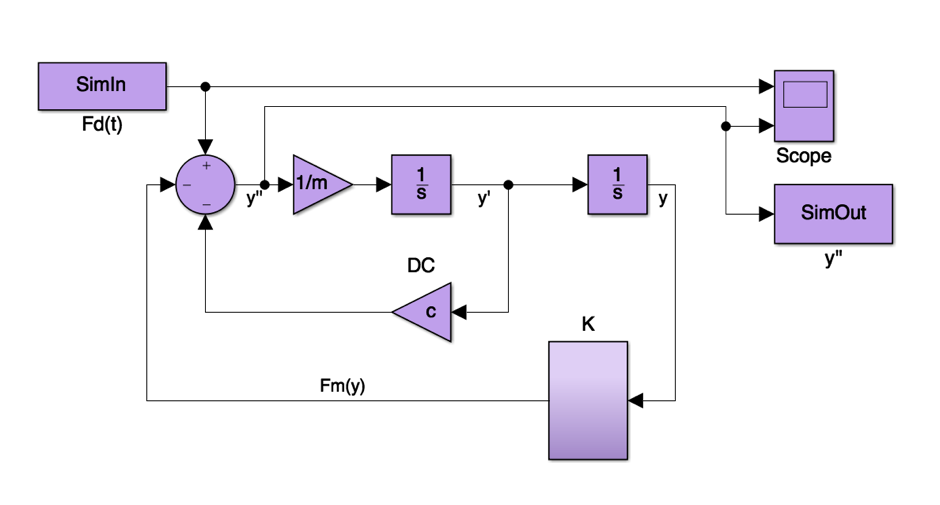
\includegraphics[width=0.8\textwidth]{Images/MatModel}
    \caption{Compared Frequency Responses with and without Squash Balls}
    \label{fig:MatModel}
\end{figure}

The constant stiffness was replaced with the subsystem used to find the 
magnetic repulsive force. \emph{SimIn} provided an interface to the MATLAB 
workspace which was used to input the driving force. Similarly, \emph{SimOut} 
exported the system output to the workspace; the acceleration of the equipment 
as a time series. Using the inverse of Equation~\vref{eq:acceleration}, the 
model output was converted into voltages so its spectra could be compared to 
the accelerometer output measured for the undamped amplifier.

Figure~\vref{fig:CoF} shows the effect of running the simulation with the 
damping coefficient at each extreme. 

\begin{figure}[h]
    \centering
    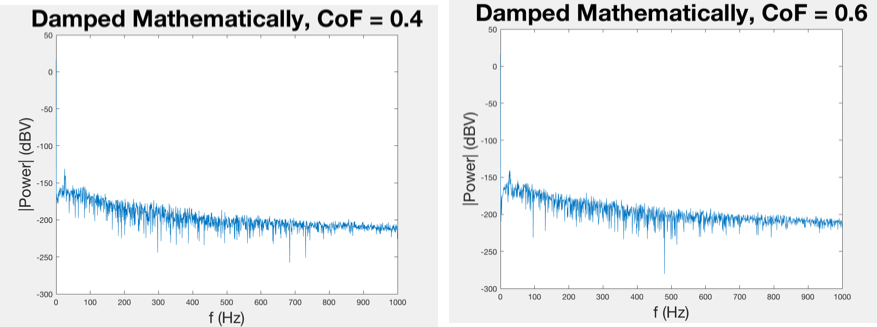
\includegraphics[width=\textwidth]{Images/MatGraph3}
    \caption{Power Output for Coefficient of Friction Extremes}
    \label{fig:CoF}
\end{figure}

In both graphs, the fundamental frequency can no longer be observed; a peak at 
around 30~\si{\hertz} is apparent however its low power and frequency that 
differs from 50~\si{\hertz} indicate that this is just noise. The noise is 
effectively identical in both cases and hence it can be concluded that the 
difference in damping coefficient across its range negligible effect. For 
further analysis, the median coefficient of friction will be used---0.5---this 
returns a damping coefficient of 198~\si{\newton\second\per\meter}.

The undamped is displayed with the simulation output damped spectrum for 
comparison between the input and output of the dynamic model in 
Figure~\ref{fig:DampedVUndamped}.

\begin{figure}[h]
    \centering
    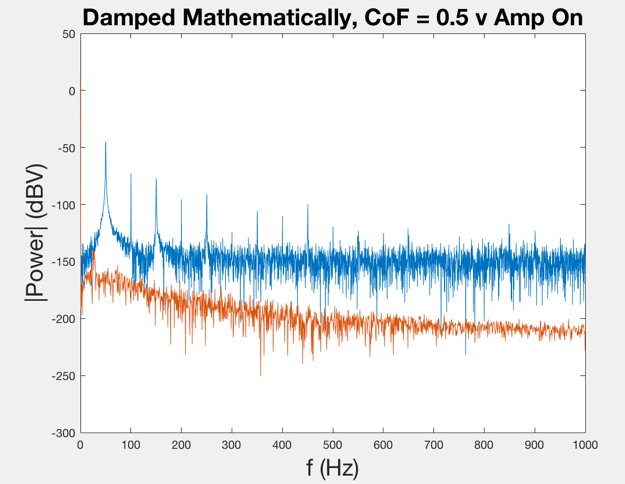
\includegraphics[width=0.8\textwidth]{Images/MatGraph4}
    \caption{Comparison of Undamped and Damped Response}
    \label{fig:DampedVUndamped}
\end{figure}

The red curve shows the simulation output; the fundamental frequency and its 
harmonics are indistinguishable from the noise. The entire signal has been 
reduced to below the noise floor of around $-140$~\si{dBV}. The noise has been 
almost completely attenuated.

The success of the footers is likely to be less significant than that of the 
model. The primary reason for this discrepancy is the value of damping 
coefficient used. Ideally, this would be found empirically; a series of 
prototypes would be produced and a similar experiment carried out to find the 
true damping coefficient.

If the footers have a fraction of the successs they have been predicted to 
have, there will be a significant improvement in sound quality. 

\section{Detail Design} \label{sec:DetailDesign}

\section{Design for Manufacture} 

DFM defines the design/engineering of a product so as to best optimise its quality whilst minimising its cost to manufacture\cite{dfm}. Factors affecting this cost include the number of off-the-shelf and machinable parts, the set-up time of required machinery, the material type, dimensional tolerances as well as secondary processes. Generally, a compromise is reached between the functional quality of a product and the cost of manufacture however, considering the current extortionate pricing of similar existing products, certain design choices have taken precedence over their implications in a manufacturing context, for the example the rails within the complex central piece are undesirable (see drawing COR080-0003).

\subsection{Bill of Materials}

\begin{table}[H]
    \centering
    \footnotesize
    \begin{threeparttable}
        \caption{Bill of Materials}
        \label{table:bom}
        \begin{tabular}{@{}clp{17em}c@{}}
            \toprule
            Item No. & Part No. & Description & Qty. \\
            \midrule
            1 & COR080-0003 & \raggedright Isofonics core piece & 1 \\
            2 & TOP080-0004 & \raggedright Isofonics top piece & 1 \\
            3 & 10MMTUNGSTENBALLS\tnote{1} & \raggedright \diameter 10~mm 
            tungsten carbide ball & 6 \\
            4 & F669-N45SH-10\tnote{2} & \raggedright \diameter 10~x~1.5~mm 
            neodymium 
            button magnet & 12 \\
            5 & PLD010-1004 & \raggedright Isofonics preloading back-stop & 1 \\
            6 & RET080-0003 & \raggedright Isofonics retainer & 1 \\
            7 & M4X20-CSK-ST\tnote{3} & \raggedright M4~x~20~mm T20 A2 c'sunk 
            screw with partial thread & 6 \\
            8 & PLD080-0003 & \raggedright Isofonics preloading crown & 1 \\
            9 & M4X20-CSK-H\tnote{4} & \raggedright M4~x~20~mm H2.5 A2 c'sunk 
            screw with partial thread & 1 \\
            10 & RET080-1002 & \raggedright Isofonics retainer bottom & 1 \\
            11 & USR080-0001 & \raggedright Isofonics removable spike & 1 \\
            12 & USR080-1002 & \raggedright Isofonics removable base & 1 \\
            \bottomrule
        \end{tabular}
        \begin{tablenotes}
            \raggedright
            \tiny
            \item[1]\url{http://www.vxb.com/10mm-Tungsten-Carbide-Bearing-Ball-0-3937-inch-Dia-p/10mmtungstenballs.htm}
            \item[2]\url{http://www.first4magnets.com/circular-disc-rod-magnets-c34/10mm-dia-x-1-5mm-thick-n45sh-neodymium-magnet-1-1kg-pull-p3633}
            \item[3]\url{http://www.westfieldfasteners.co.uk/A2_ScrewBolt_PinTXCsk_M4.html}
            \item[4]\url{http://www.westfieldfasteners.co.uk/A2_ScrewBolt_SHCsk_M4.html}
        \end{tablenotes}
    \end{threeparttable}
\end{table}

\subsection{Off-The-Shelf Parts}
Due to the complex geometry required from our design, only few components may be bought in, namely (per mount);  six �10mm tungsten carbide ball bearings, six \diameter 10 x 1.5 mm neodymium magnets, six M4 by 20 mm AISI A2 steel countersunk Torx security screws and one M4 by 20 mm countersunk hex socket with partial thread. These components are readily available excluding the tungsten carbide ball bearings which must be sourced from a specialist supplier.
Table~\ref{table:bom} details potential sources for the aforementioned parts and the quantity required per mount.

\begin{table}[h]
	\centering
	\caption{Costing}
	\begin{tabular}{@{}rp{9em}p{9em}rrr@{}}
		\toprule
		Item No. & Part No.  & Qty. & �/Piece & � Total \\
		\midrule
		1 & COR080-0003 & 1 & --- & --- \\
		2 & PLD080-0003  & 1 & --- & --- \\
		3 & PLD010-1004  & 6 & --- & --- \\
		4 & F669-N45SH-10 (first4magnets) & 12 & 0.30 & 3.6  \\
		5 & 10MMTUNGSTENB ALLS (VXB Bearings) & 6 & 20.30 & 243.60 \\
		6 & TOP080-0004A  & 1 & --- & --- \\
		7 & RET080-0003 & 1 & --- & --- \\
		8 & M4X20-CSK-ST (westfieldfasteners) & 1 & 0.09 & 0.09 \\
		9 & M4X20-CSK-H (westfieldfasteners) & 1 & 0.04 & 0.04 \\
		10 & USR080-0001 & 1 & --- & --- \\
		11 & RET080-1002  & 1 & --- & --- \\
		12 & USR080-1002 & 1 & --- & --- \\
		\bottomrule
\end{tabular}
\label{table:costs}
\end{table}

\subsection{Primary Processes}

All parts are to be machined using a 3 axis CNC mill excluding the central piece (see drawing COR080-0003), which requires 4 axis machining. 4 axis machining is more expensive but allows for more intricate designs by using a 4th axis to reposition the part between 3 axis operations, a feature required for this design\cite{cnc}. Forging was considered as a method of manufacture but was dismissed for the following reasons; the large expenditure involved in machinery, dies, tools and personnel are only justifiable for large scale production and the die accuracy required to forge the most complex pieces is likely unachievable\cite{Forging}. In the interest of reducing manufacturing cost, for which the complex geometry of the core piece is largely responsible, it is possible that that piece be machined in separate parts that are later joined to avoid the machining of reverse chamfers as shown in Figure~\ref{fig:core}.

\begin{figure}[h]
   \centering
   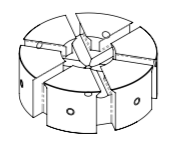
\includegraphics[width=0.3\textwidth]{Images/core}
   \caption{Core}
   \label{core}
\end{figure} 

Cost is substantially driven by time; time to remove material in the machining process as well as set-up time of the machine itself\cite{SetUp}. Conveniently, our design is highly symmetrical meaning time and money is saved through lacking the need of a complex orienting mechanism given that the part's orientation prior to machining is irrelevant.

Finally, the volume of production is of great importance; with too small a batch size, set up costs and jig production costs become impractical and with too large a batch, storage costs pose a problem for a product of which the market response is not easily predictable. Considering the high cost and exclusive appeal of this product, low volume batch production in the order of 100 is appropriate so as to eliminate any unnecessary storage costs and allow adequate response to market needs. Specifically a volume of 600 pieces has been defined simply because it is within the correct order of magnitude and is divisible by three; the mounts are expected to be sold in groups of three.

\subsection{Secondary Processes}

A range of finishes best suited to individual parts have been chosen based on 
its functionality and location. A relatively cheap 2B (basic smooth) finish is 
to be applied to the stainless steel core so as to prohibit unnecessary 
expenditure considering the part shall not be seen by the customer whilst 
ensuring a path of minimal friction exists for the moving ball bearings. 
Additionally, the standard aluminium mill finish is rough and so all internal 
aluminium pre-loading pieces are to be brushed in the direction the piece 
travels so as to limit the amount of wear. Furthermore, the external retainer 
is to be brushed in concentric circles to give an attractive finish and hide 
any scratches. A 2J finish is to be applied to all other external stainless 
steel pieces since it is cheaper to produce than polishing and is practical in 
that it is resistant to scratches whilst being aesthetically 
pleasing.\cite{Finishes}

All parts are to be machined at fine linear and angular tolerances of +/-0.1mm 
and +/-$1\,^{\circ}\mathrm{}$ respectively to ensure the overall quality of the 
product. However there exists opportunity for optimisation within this section; 
in the interest of reducing cost, it was concluded that the rails contained in 
the core piece are the only parts to be machined to a high tolerance since they 
are to fit plush to the bearings; all other parts may be machined to a coarser, 
and therefore cheaper, tolerance.

\subsection{Manufacture Costs} \label{sec:ManCosts}
Table \ref{table:costs} details the cost of off-the-shelf parts and machining 
per mount, totalling �y. It is worth noting that the off-the-shelf pricing has 
been quoted for relatively low volume purchases, specifically within the range 
100-200 pieces, and would decrease for larger scale production as to be used 
for this product; a batch volume 600 of pieces.

\section{Design for Assembly} 
\subsubsection{Jig Design}
Due to the small scale of our product, hand assembly is required. Considering the complexity of the design and physical impracticality of overcoming the repulsive magnetic forces during its assembly, a jig has been designed, as shown in drawings JIG080-0001 and JIG080-1001, with full accompanying assembly instructions (see Isofonics Assembly Instructions ISO080-INS).

\begin{figure}[h]
    \centering
    \subfloat[Assembly Jig Base]{{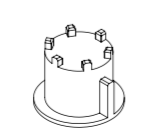
\includegraphics[width=0.4\textwidth]{Images/jigbase} }}%
    \qquad
    \subfloat[Assembly Jig Sleeve]{{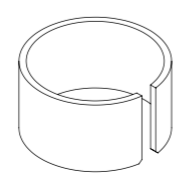
\includegraphics[width=0.3\textwidth]{Images/jigsleeve} }}%
    \caption{Assembly Jig Components}
    \label{fig:JigAssembly}
\end{figure}

\subsection{Assembly Costs} \label{AssemCosts}
Considering the assembly jig is to be re-used indefinitely, its cost is negligible within the context of the product's assembly. Assembly costs are then only defined by the time taken to manually assemble the device and the cost of manual labour which can be estimated at 2 minutes and \textsterling8/hr respectively. This equates to a total of \textsterling0.27 per piece.

\section{Design for Sustainability} 
\section{Commercial Considerations} 

\subsection{Brand Development and Competitor Analysis}
With the intention of establishing the design in the market, a brand identity 
was essential. Through several brainstorming sessions, the team agreed on the 
name ?Isofonics.? It was important to review the current market leaders, 
Stillpoints and Nordost, with their relevant products. Nordost primarily 
manufactures Hi-Fi audio cables but recently introduced additional products for 
resonance and power control. Namely, their ?Sort Kone,? acts as a vibration 
drain with a mechanical diode effect to prevent external vibrations from 
travelling up through the cone. Similarly, 3 cones are recommended per device 
but they offer 3 types of cone, each made from different materials. The most 
expensive is made from titanium and utilises ceramic bearings, retailing at 
�349.99 per cone. The 3 mounts do not necessarily have to be the same and the 
user may find it more beneficial to use a mixture. (See Figure 3) [7]
 
\subsection{Stillpoints Patent Check}
 
The Stillpoints patent details the design of a \lq{device for the control of 
vibrations comprising a retainer resting on a base and a plurality of bearings 
disposed within the retainer}\rq \cite{Stillpoints}within which \lq{the 
bearings are arranged in at least two layers}\rq \cite{Stillpoints}. It alludes 
to multiple alternative designs including an \lq{embodiment}\rq in which 
magnetic fields are employed, however differently to the usage detailed in our 
design. After studying the official claims made at the end of the patent it is 
concluded that in not featuring layers of bearings and using opposing magnetic 
fields as the main damping method, our design differs significantly from the 
design and alternatives claimed by Stillpoints.

\textbf{It is worth noting this is a US patent and is not filed with the 
European Patent Office and so only stands to limit sales within the US}
 
\subsubsection{Parallels with Stillpoints}
The following details the main claim made by Stillpoints and highlights areas 
of concern:

\lq{A device for the control of vibrations comprising:
\textbf{a retainer}, the retainer constructed and arranged to rest upon a base, at least a \textbf{portion of the base defining a substantially flat surface}; and \textbf{a plurality of bearings disposed within the retainer, the bearings arranged in a first layer and a second layer}, the second layer disposed on the first layer, the first layer
comprising three or more bearings, and the second layer comprising at least one bearing, each bearing in
the first layer constrained on its bottom by only the substantially flat surface of the base, on its side by the
retainer, the bearings in the first layer supporting the at least one bearing in the second layer, the retainer defining a surface which is in substantially tangential contact with the bearings in the first layer}\rq\cite{Stillpoints}.

It is clear that the main claim focuses on the use of layers of bearings, in this way, our design is fundamentally different. Since our design differs from that outlined in the main claim, all further claims based on the first are irrelevant. An element of originality of our design lies in the use of magnets which is not mentioned at all within the official claims section of the patent.

The use of magnetic fields is mentioned during the preamble and is as follows:

\lq{In some embodiments the first base member 119 and second base member 123 may have opposing magnetic fields.}\rq\cite{Stillpoints}

\begin{figure}[h]
    \centering
    \subfloat[Stillpoints Mechanism Diagram]{{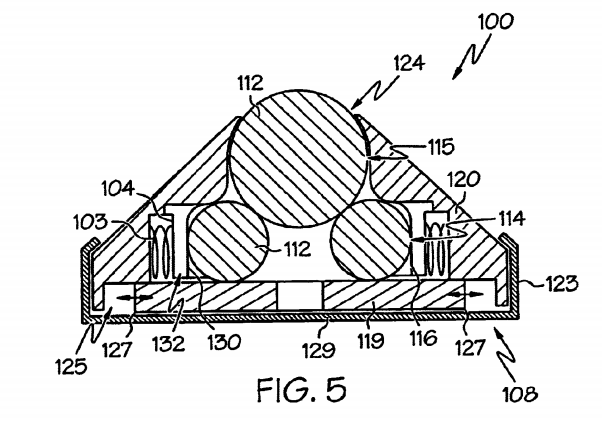
\includegraphics[width=0.4\textwidth]{Images/Stillpoints} }}%
    \qquad
    \subfloat[Group 25 Mechanism Diagram]{{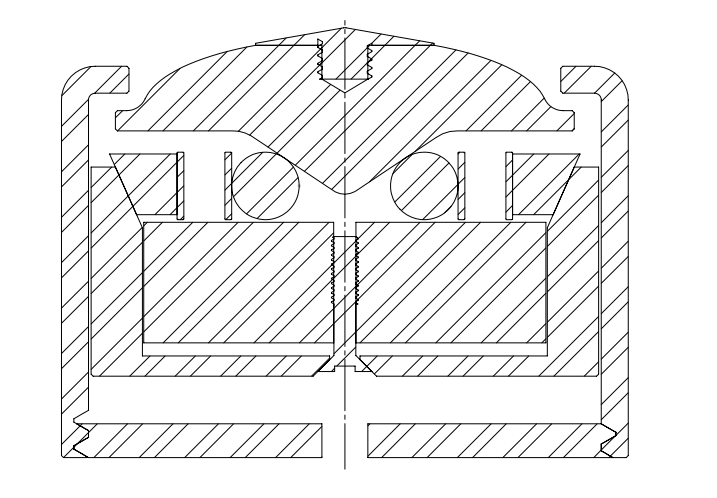
\includegraphics[width=0.4\textwidth]{Images/Group25} }}%
    \caption{Stillpoints Mechanism Comparison}
    \label{fig:Patent}
\end{figure}
As can be seen from Figures 1 and 2 , this comment is entirely unrelated to the use of opposing magnetic fields to essentially replace the spring mechanism shown above and consequently does not affect our design.

Figure ~\ref{fig:Patent}

\subsubsection{Points of Originality}
\begin{itemize}
    \item Use of \textbf{opposing magnetic fields} for lateral damping as 
    opposed to springs
    \item \textbf{Cone with retaining flange} replacing layers of bearings
    \item \textbf{Pre-loading mechanism} in which a screw in tension moves a 
    fixed magnet decreasing its distance from the bearing magnet thus 
    increasing the strength of the system---adjustable for a variety of masses.
\end{itemize}

\subsection{Marginal Costs}
With respect to production costs, margins of 100\% for product distribution, 100\% for retail and 35\% for profit are to be met. Given that machining and assembly costs total �x (see section \ref{sec:ManCosts}) and �y (see section \ref{sec:AssemCosts}) per piece respectively, the product's cost of production is �r per piece. The aforementioned product margins then dictate a retail price of �(1.35 * r).

\section{Discussion} 
\subsection{Specification Fulfilment}
\subsubsection{User Requirement Specification Tree}
With reference to the URS tree, the final proposal incorporated a cone with a retaining flange which held the magnets in place whose separation was altered in order to accommodate a range of masses. The four degrees of freedom were thus defined by all translational motion and free rotation. As described earlier in the report, the magnet behind the bearing is moved while the other is fixed and the preloading mechanism allowed the user to adjust the position of the fixed magnet. Namely, the crown element moved the back stops for the fixed magnet inward as a single preloading screw was tightened. 

The requirement for a rigid load path was integral to the performance of the 
damping mechanism. The interaction between the magnets and the spherical 
bearings in conjunction with the hardness of their material clearly diminished 
the excess mechanical vibrations generated by microphonic effects as 
demonstrated by the graphs produced by the dynamic model. However, the data 
yielded during the experiment which was then inputted to the simulation, did 
not totally reflect the execution of the design. Employing the squash balls as 
a method of dampening the noise produced by the amplifier did validate the 
concept but this could be supported further by utilising a prototype and later 
determining the damping coefficient for different loads empirically. If these 
results demonstrated a fraction of the model?s success, then the mount can 
still be confidently viewed as a success. 

The Hi-Fi equipment must only rest on 3 footers to prevent further resonances and heating in the arrangement. If another was used, it would either prove redundant or induce further noise. The cone provided a single point of contact which in turn meant that 3 footers were needed to support one piece of equipment. Partnered with the large base plate, this guaranteed that the mounts would not slip and the system was amply stable. For this reasoning, the footers would be sold in sets of three.

A 2-D finite element analysis software was used to model the magnetic flux 
distribution within the mount. Although it was concluded that there was no 
additional interference or damage to the Hi-Fi system, ideally a 3-D finite 
element analysis software would better determine whether the separation 
distance or the grade of magnet needed to be amended.

\subsection{further developments}
There is great potential for further work and like Nordost, a family of 
products adapted to support heavier devices such as loudspeakers could also be 
developed by changing the material for the spherical bearings or by varying the 
magnetic field strength to yield a new damping factor and related coefficient. 
A companion phone application which enables the user to adjust the preload for 
a desired condition could also replace the preloading graphs provided by the 
parametric model. Machining could be improved by optimising tolerancing for the 
tracks and will thus increase profit margins and set the product aside from the 
mentioned competitors.

\section{Conclusion}

\section{References}
\printbibliography

% Appendicies
\cleardoublepage
\appendix
\section{Project Plan and Members' Contributions} 
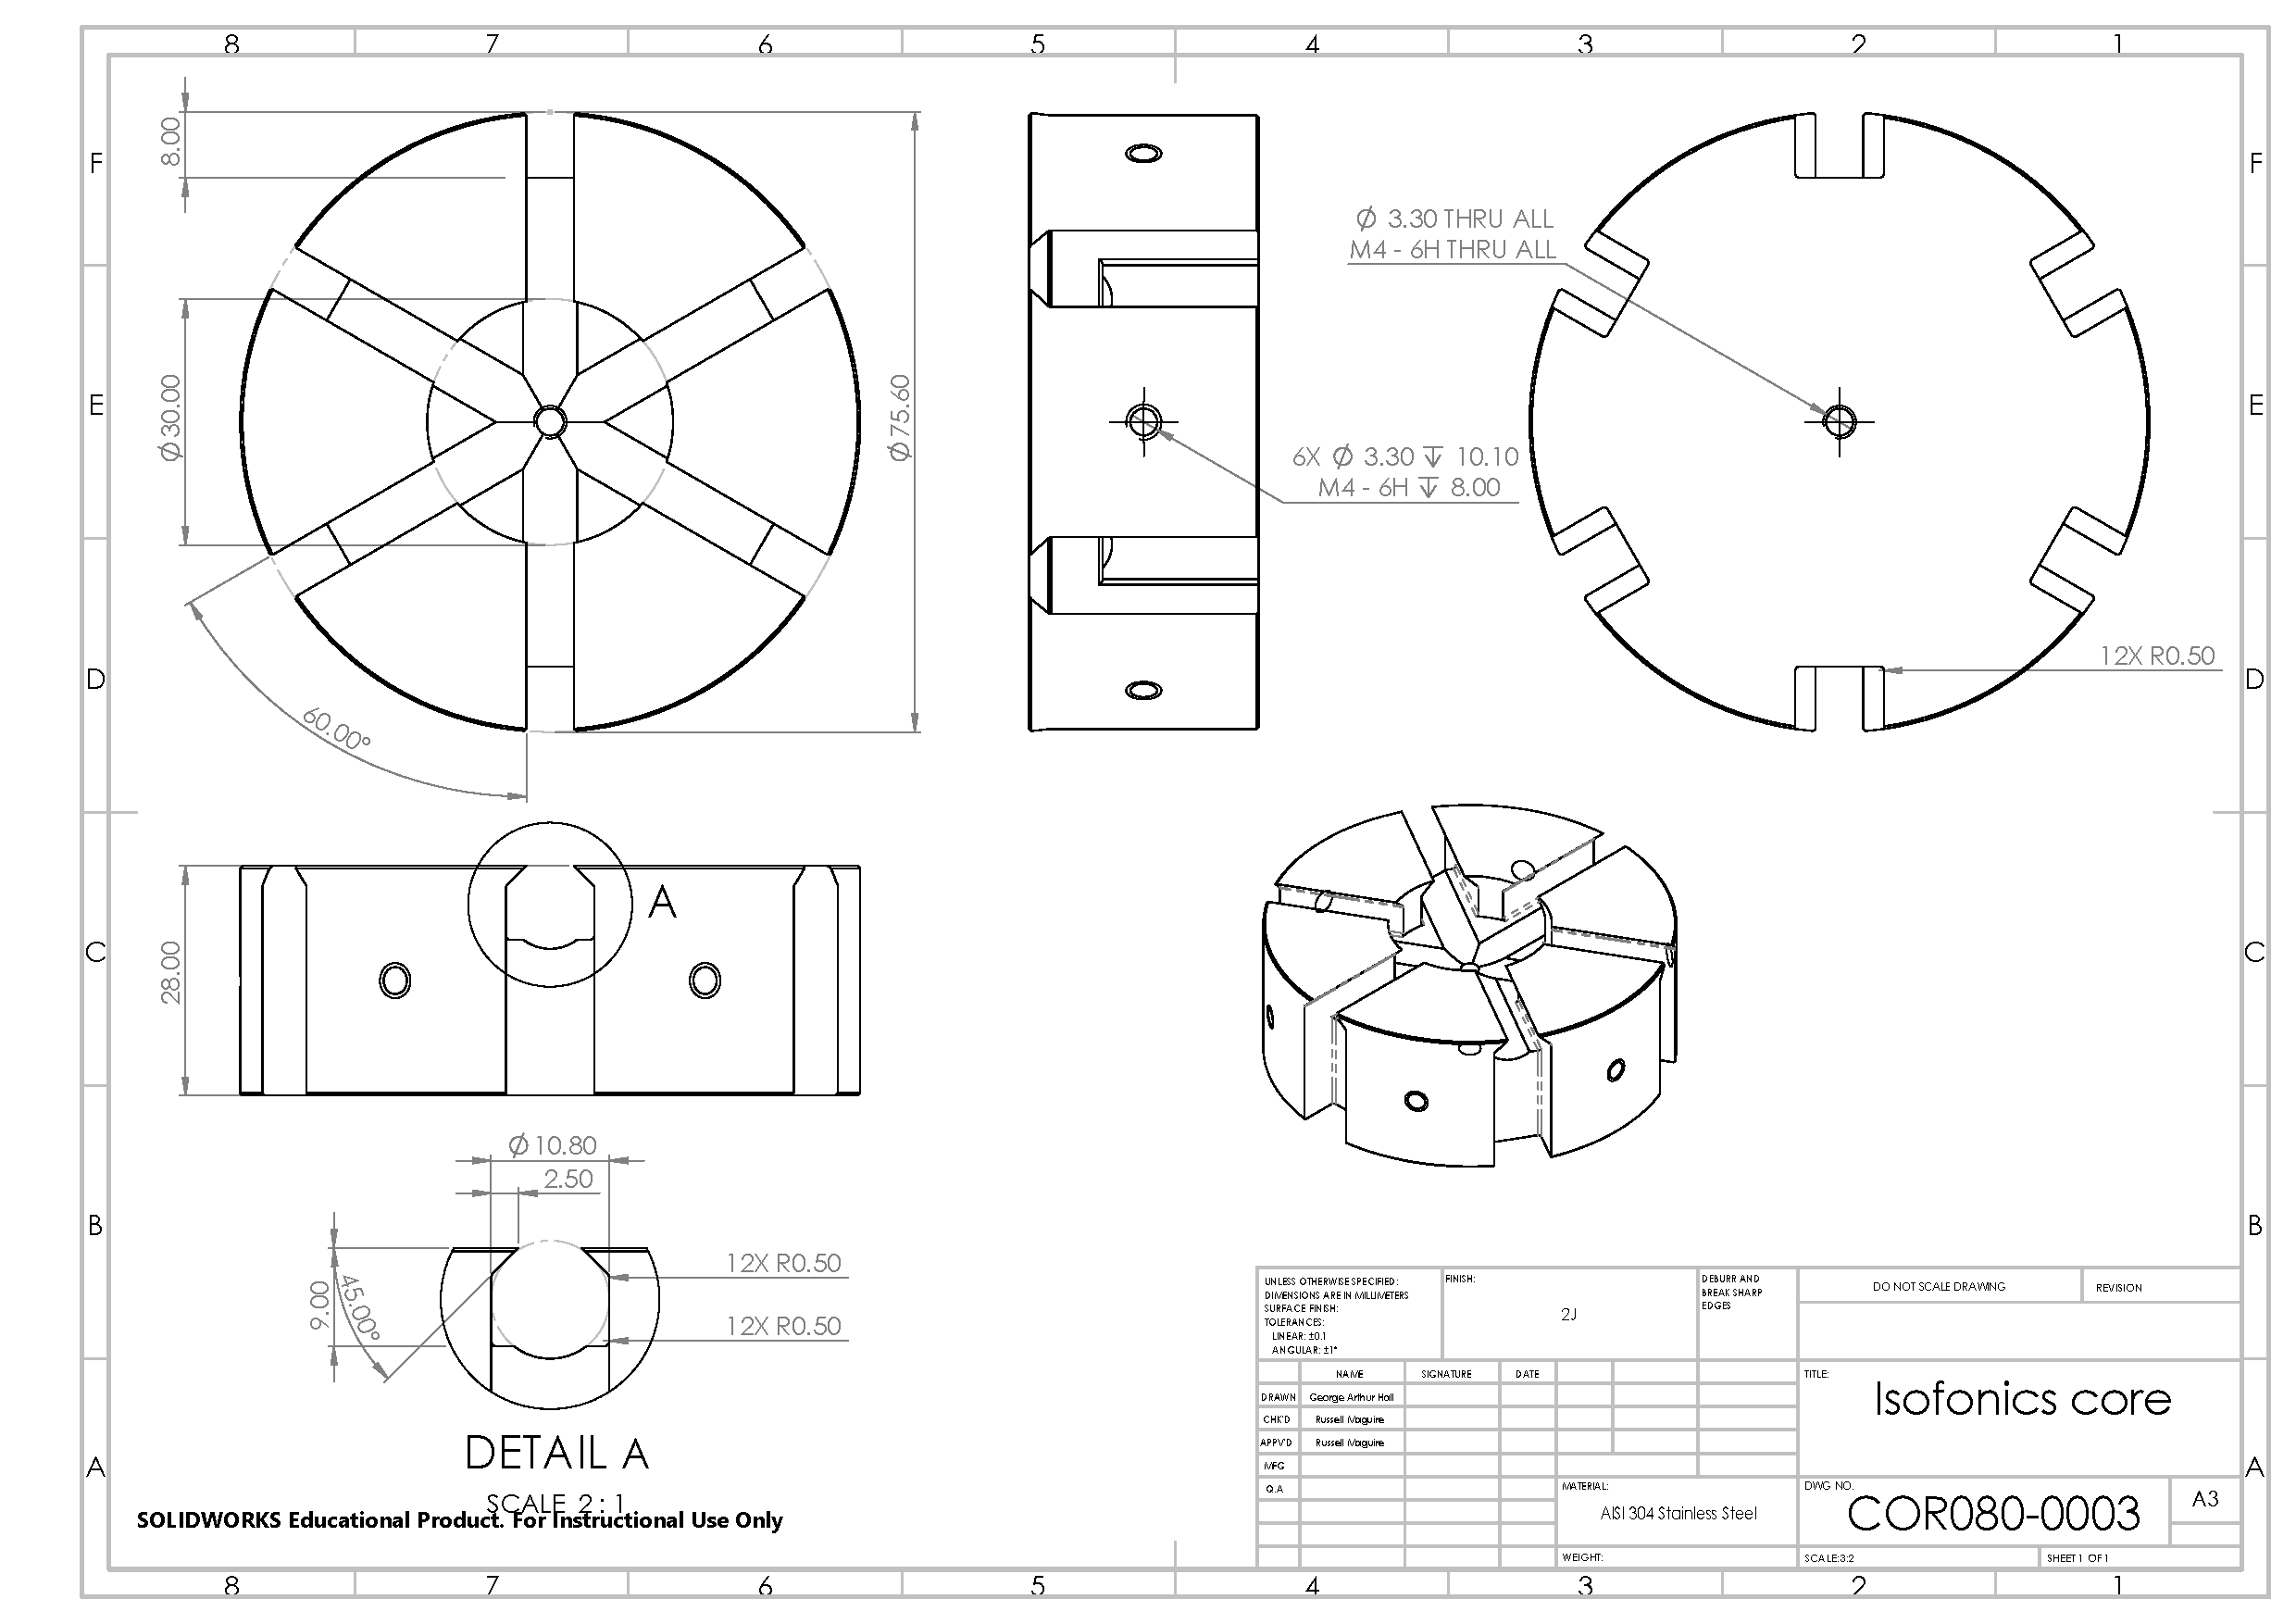
\includepdf[pages=-,fitpaper=true]{Images/Drawings/COR080-0003.PDF}
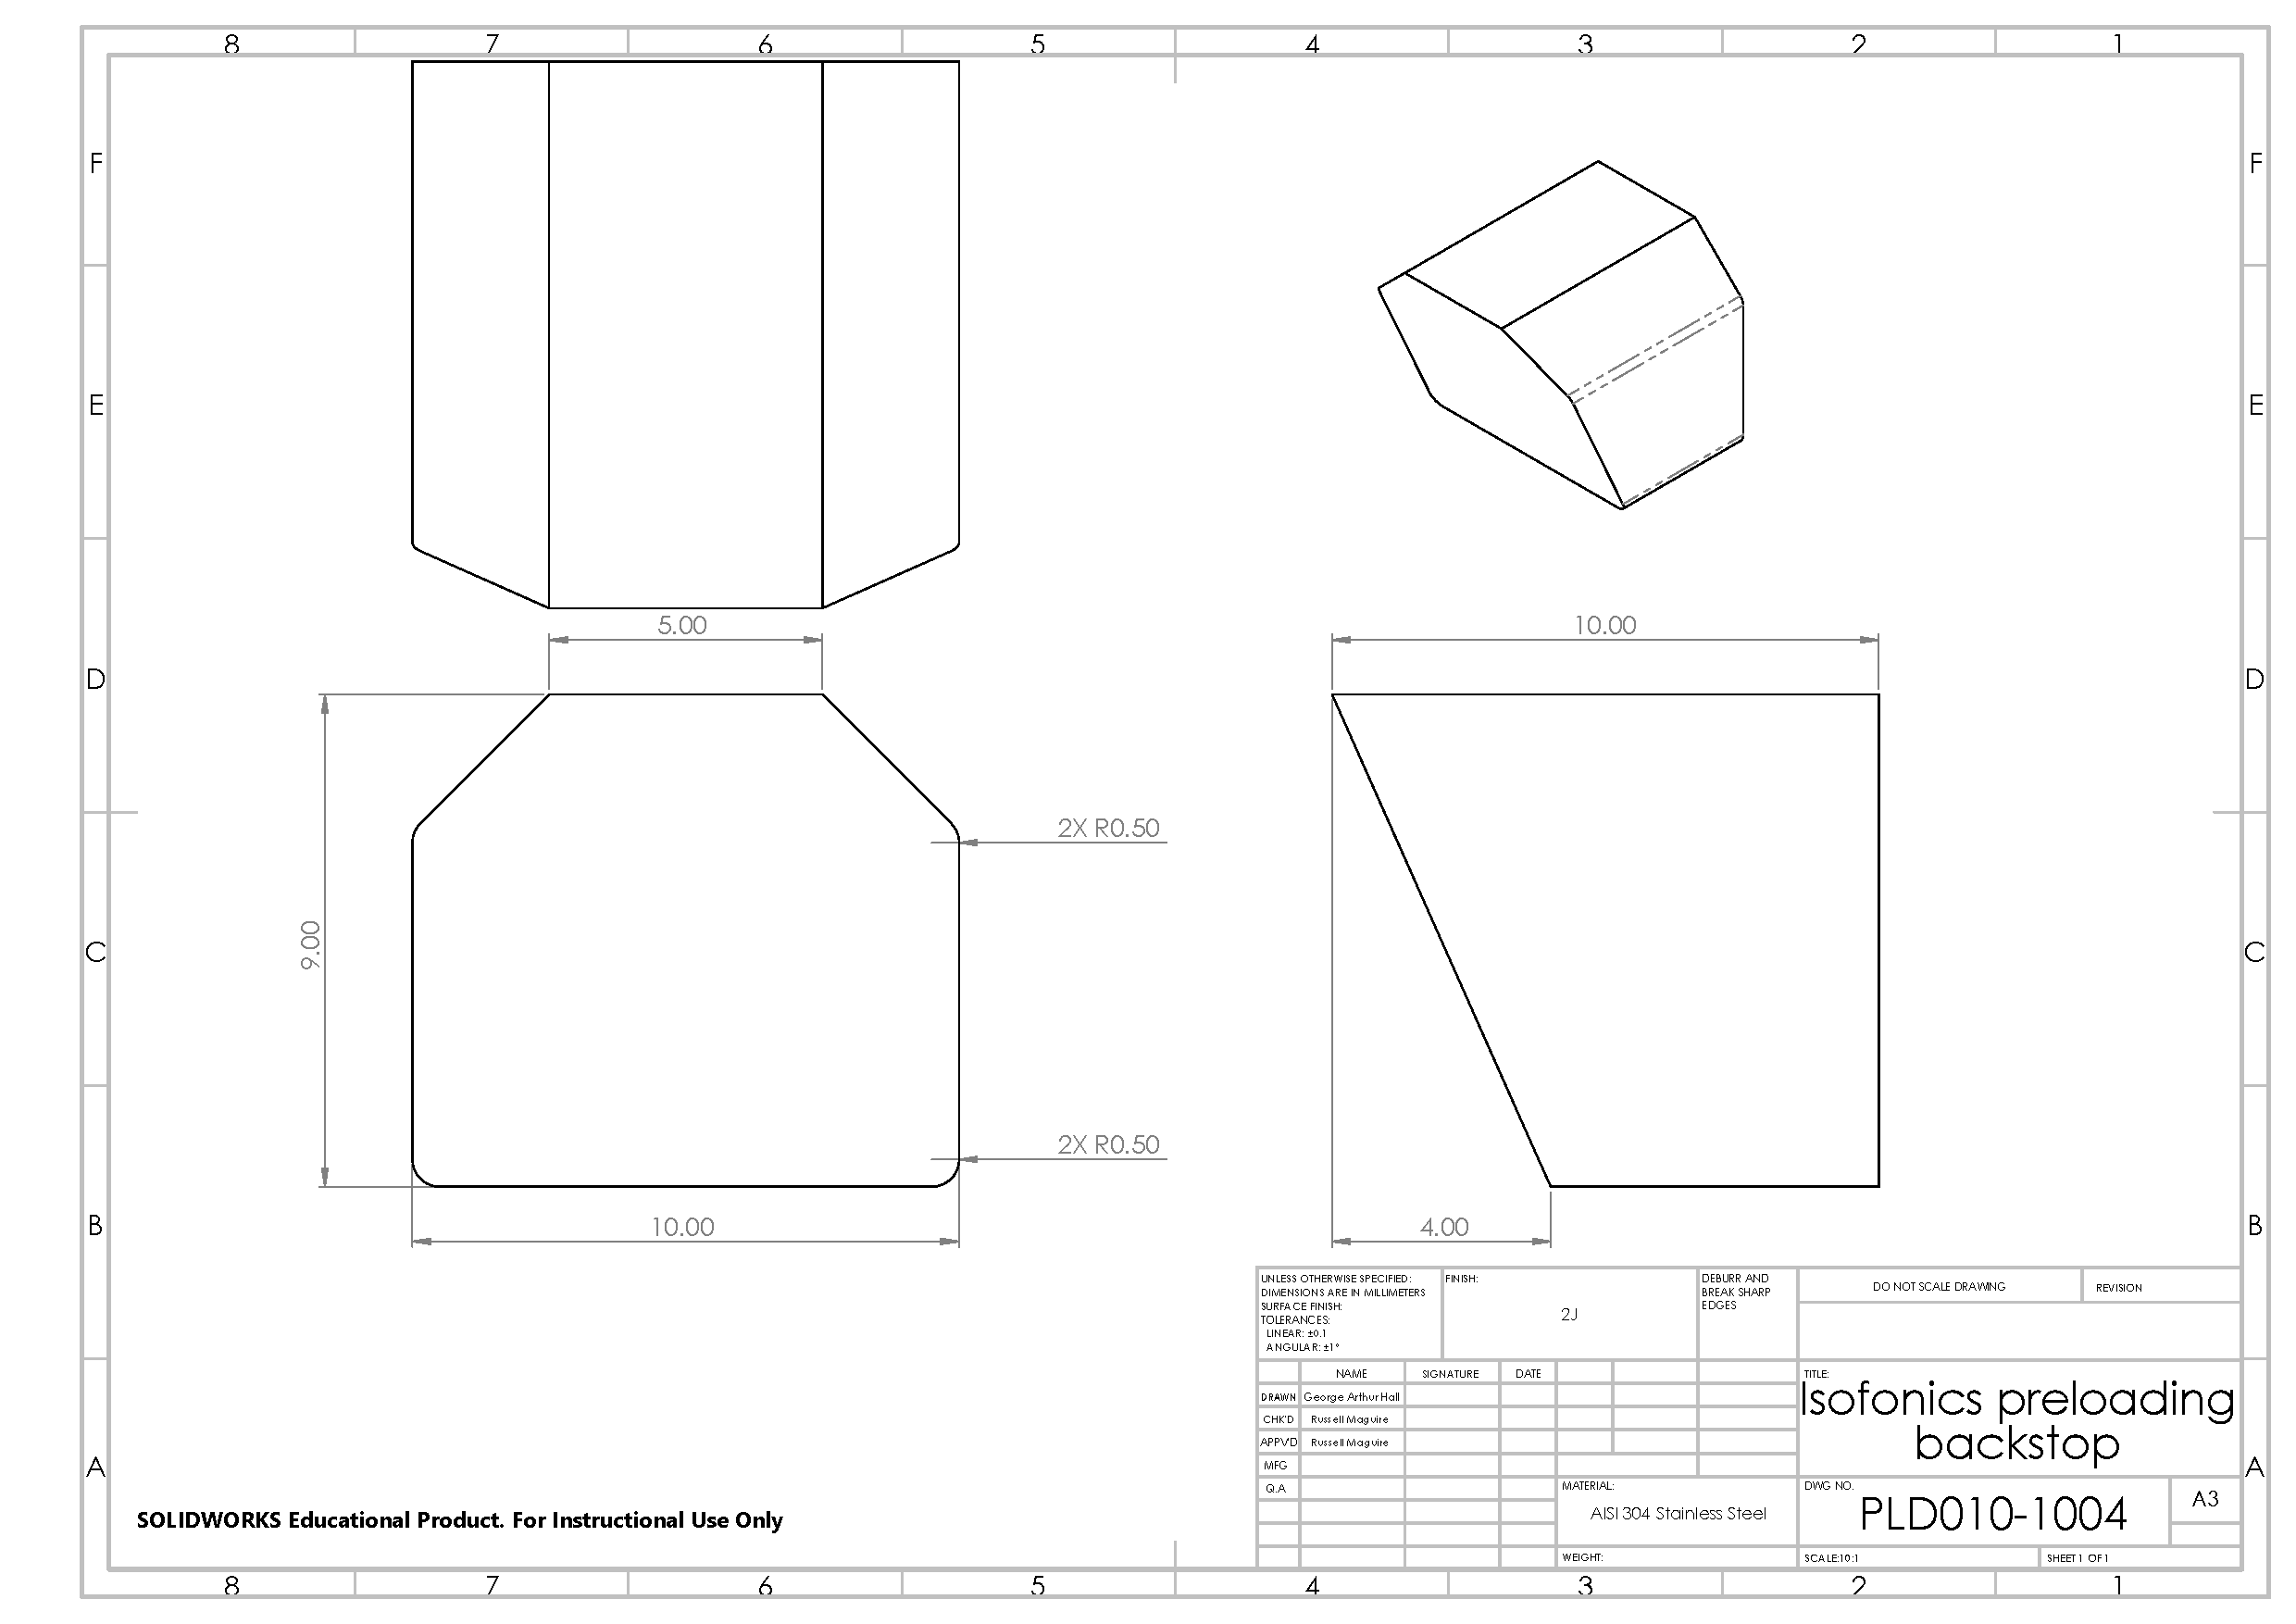
\includepdf[pages=-,fitpaper=true]{Images/Drawings/PLD010-1004.PDF}
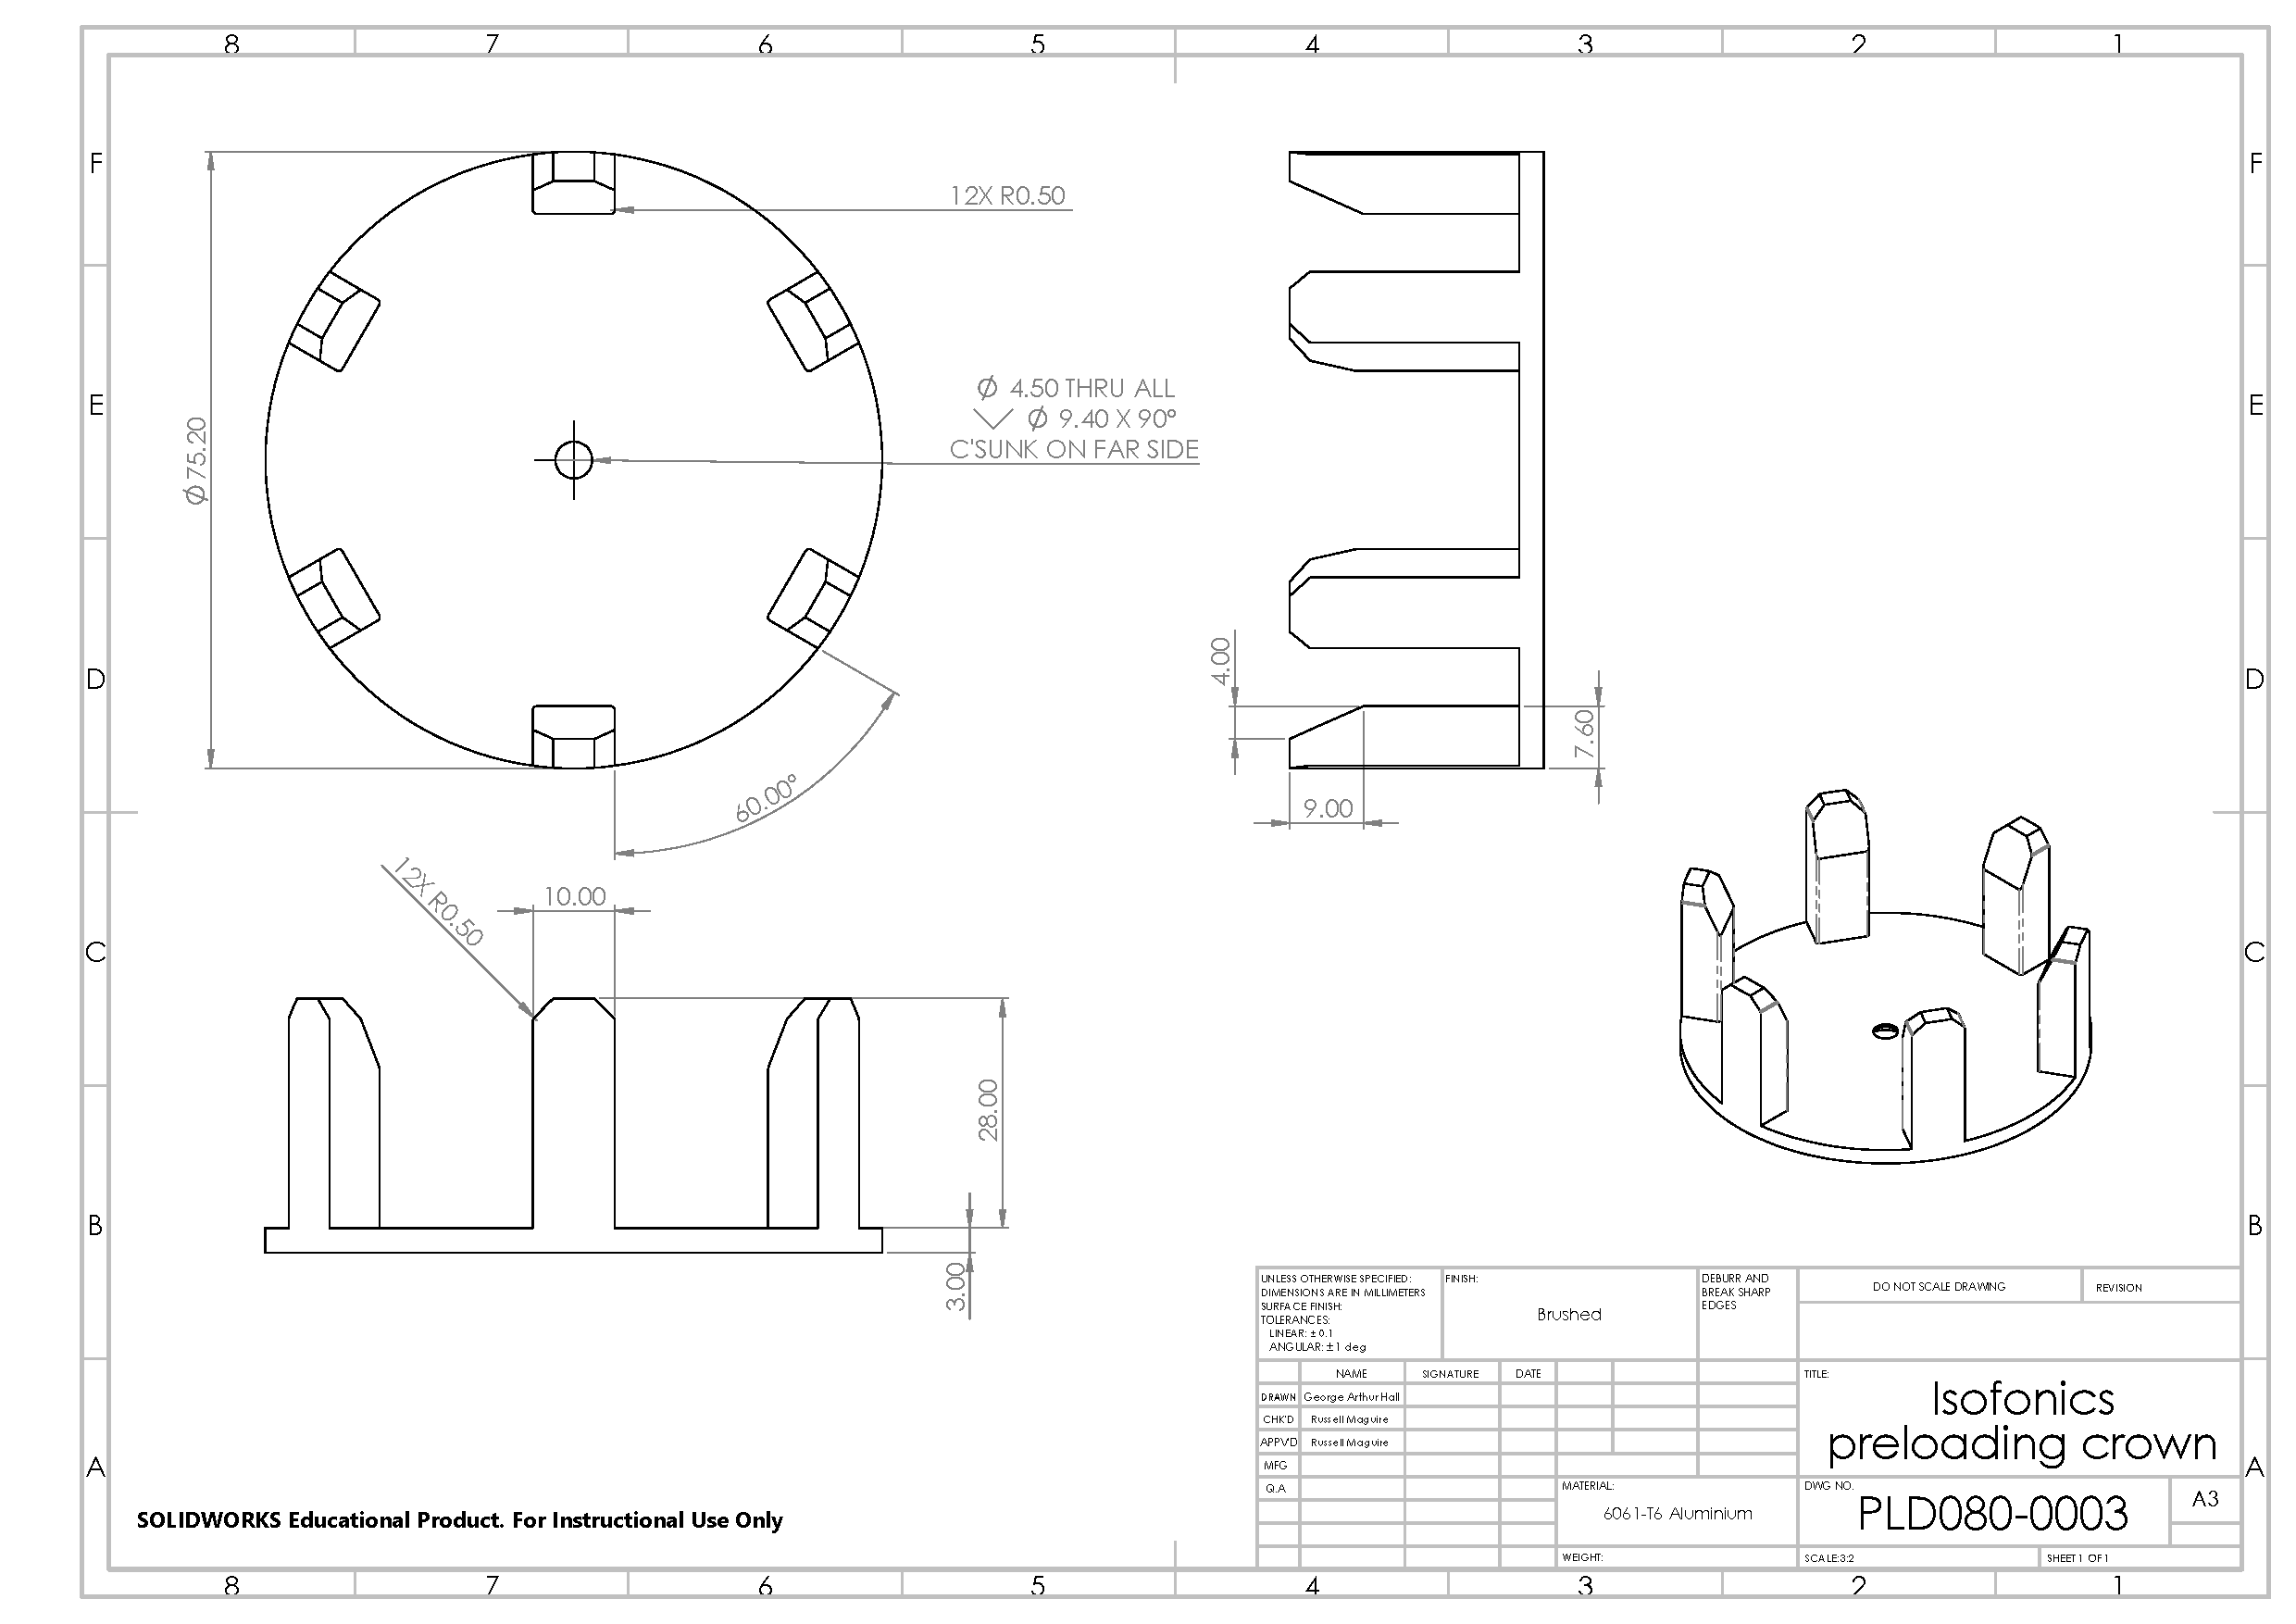
\includepdf[pages=-,fitpaper=true]{Images/Drawings/PLD080-0003.PDF}
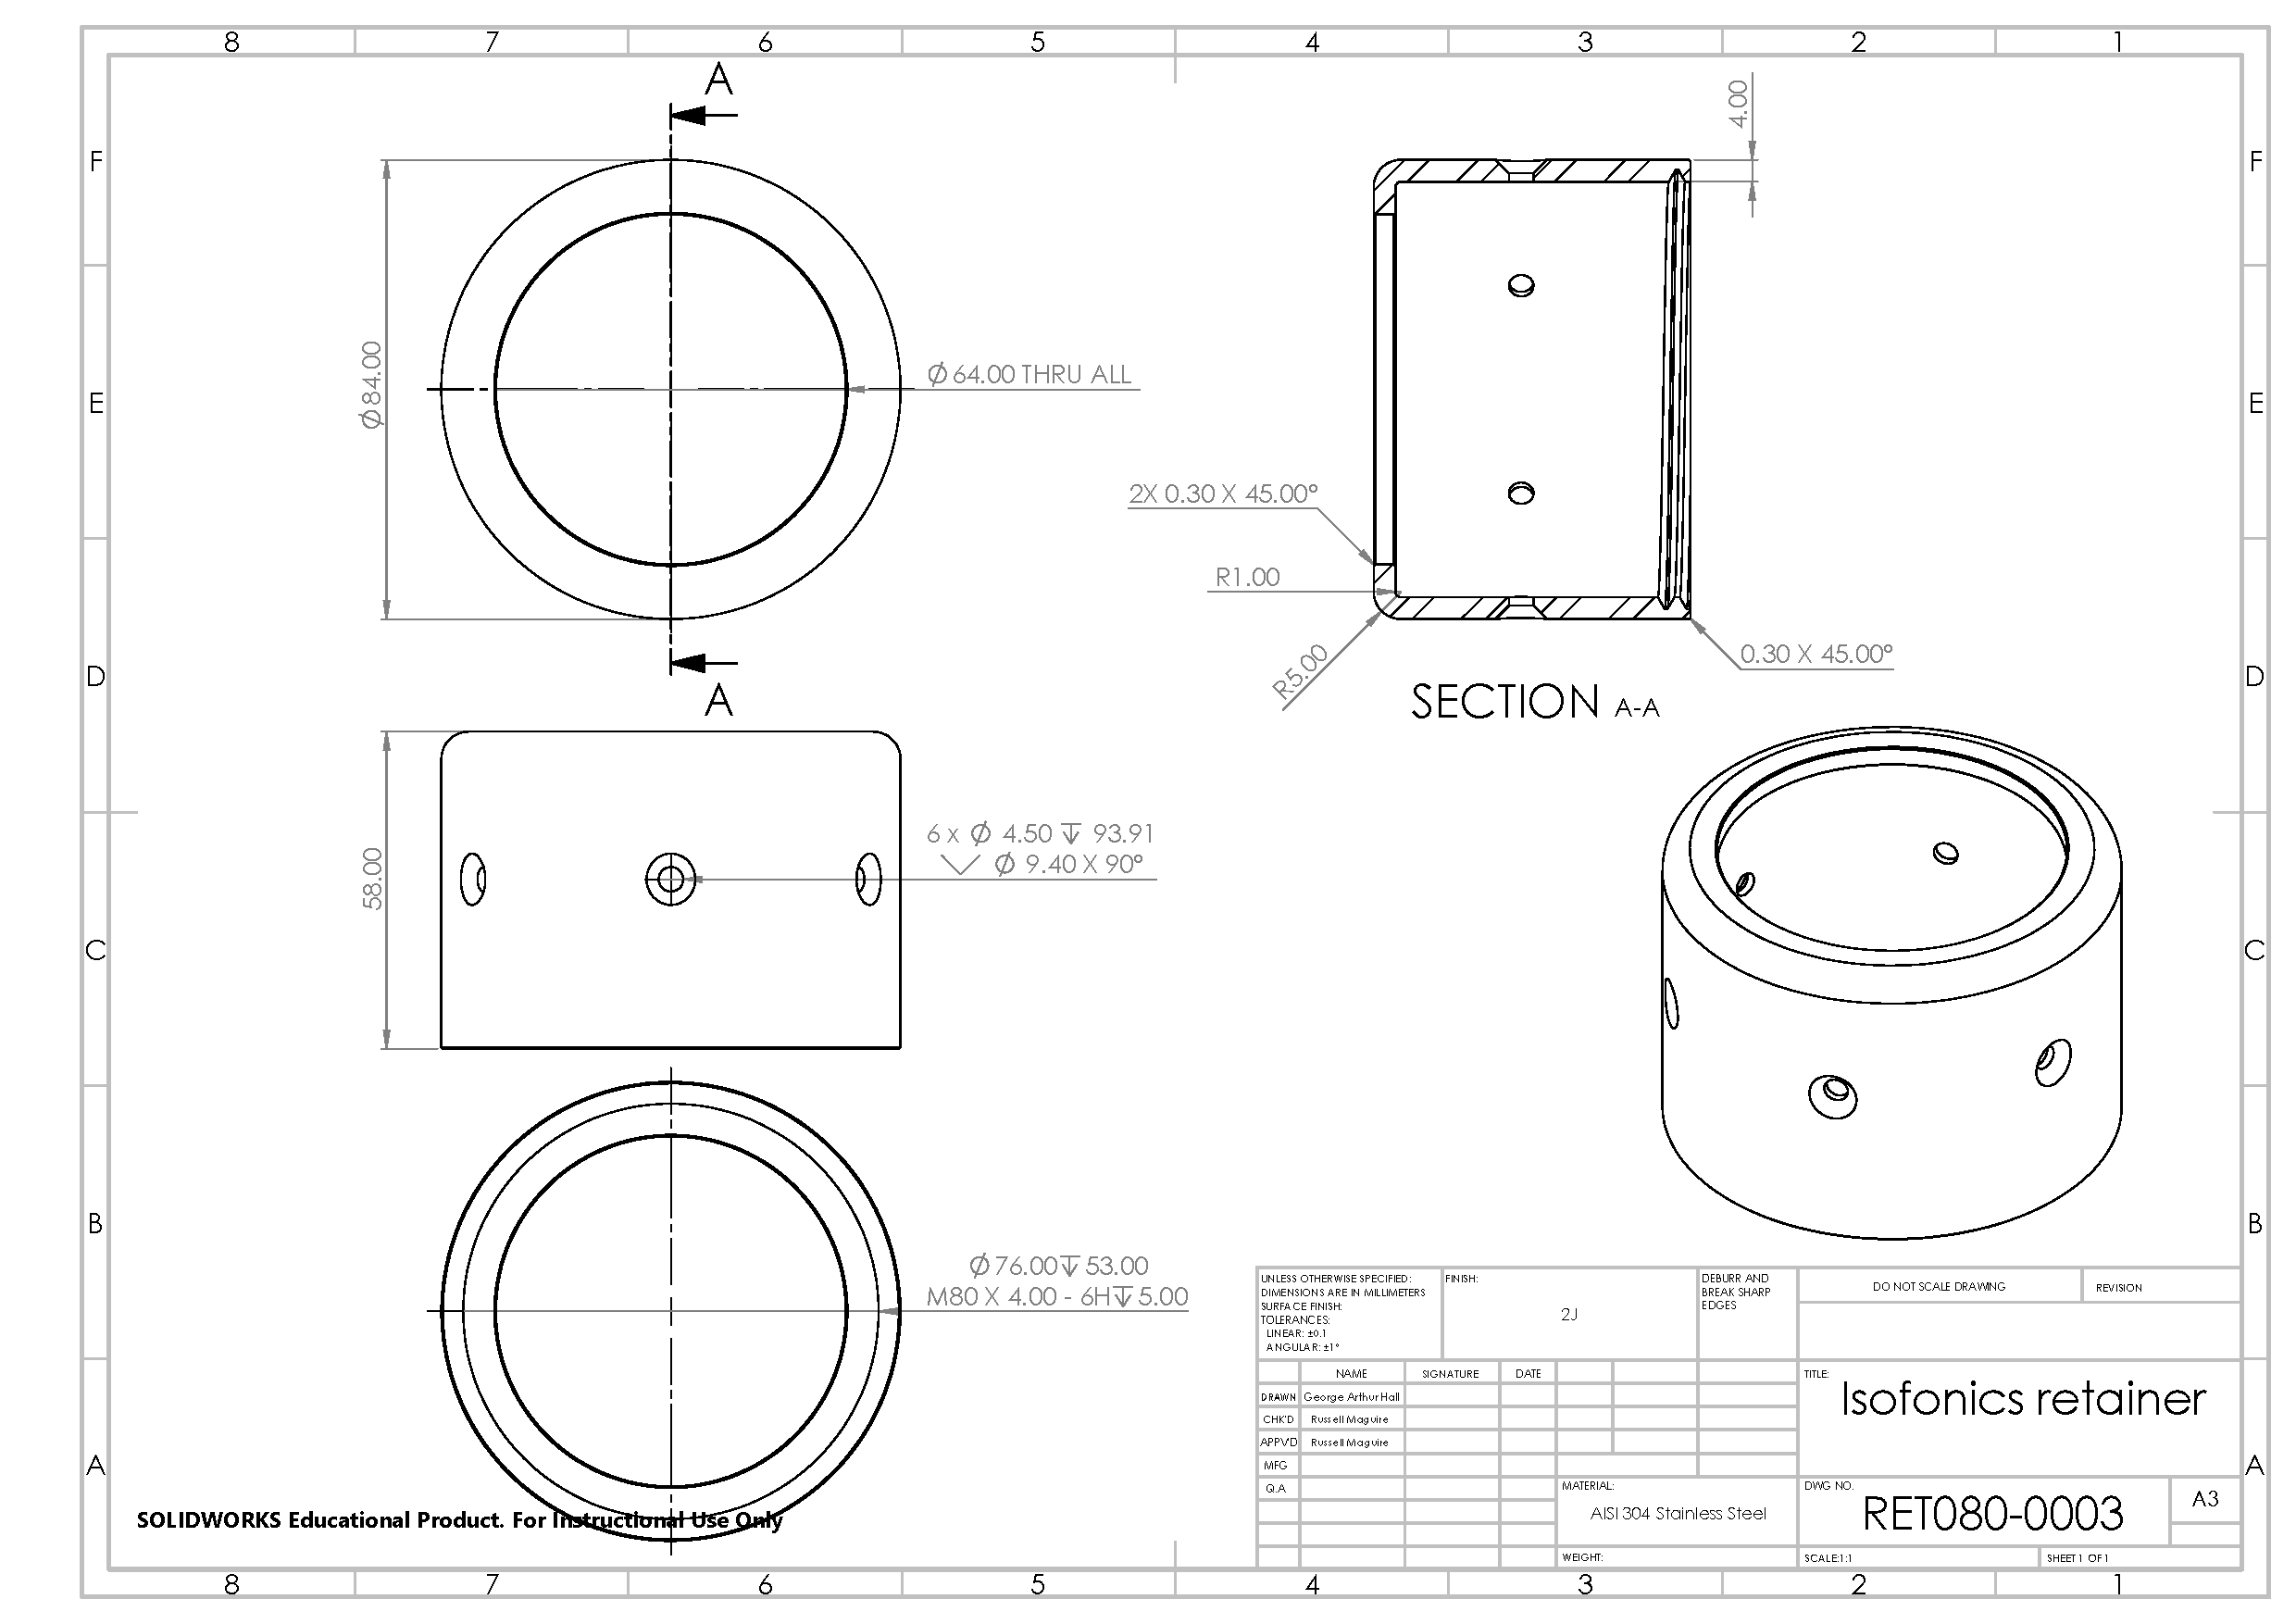
\includepdf[pages=-,fitpaper=true]{Images/Drawings/RET080-0003.PDF}
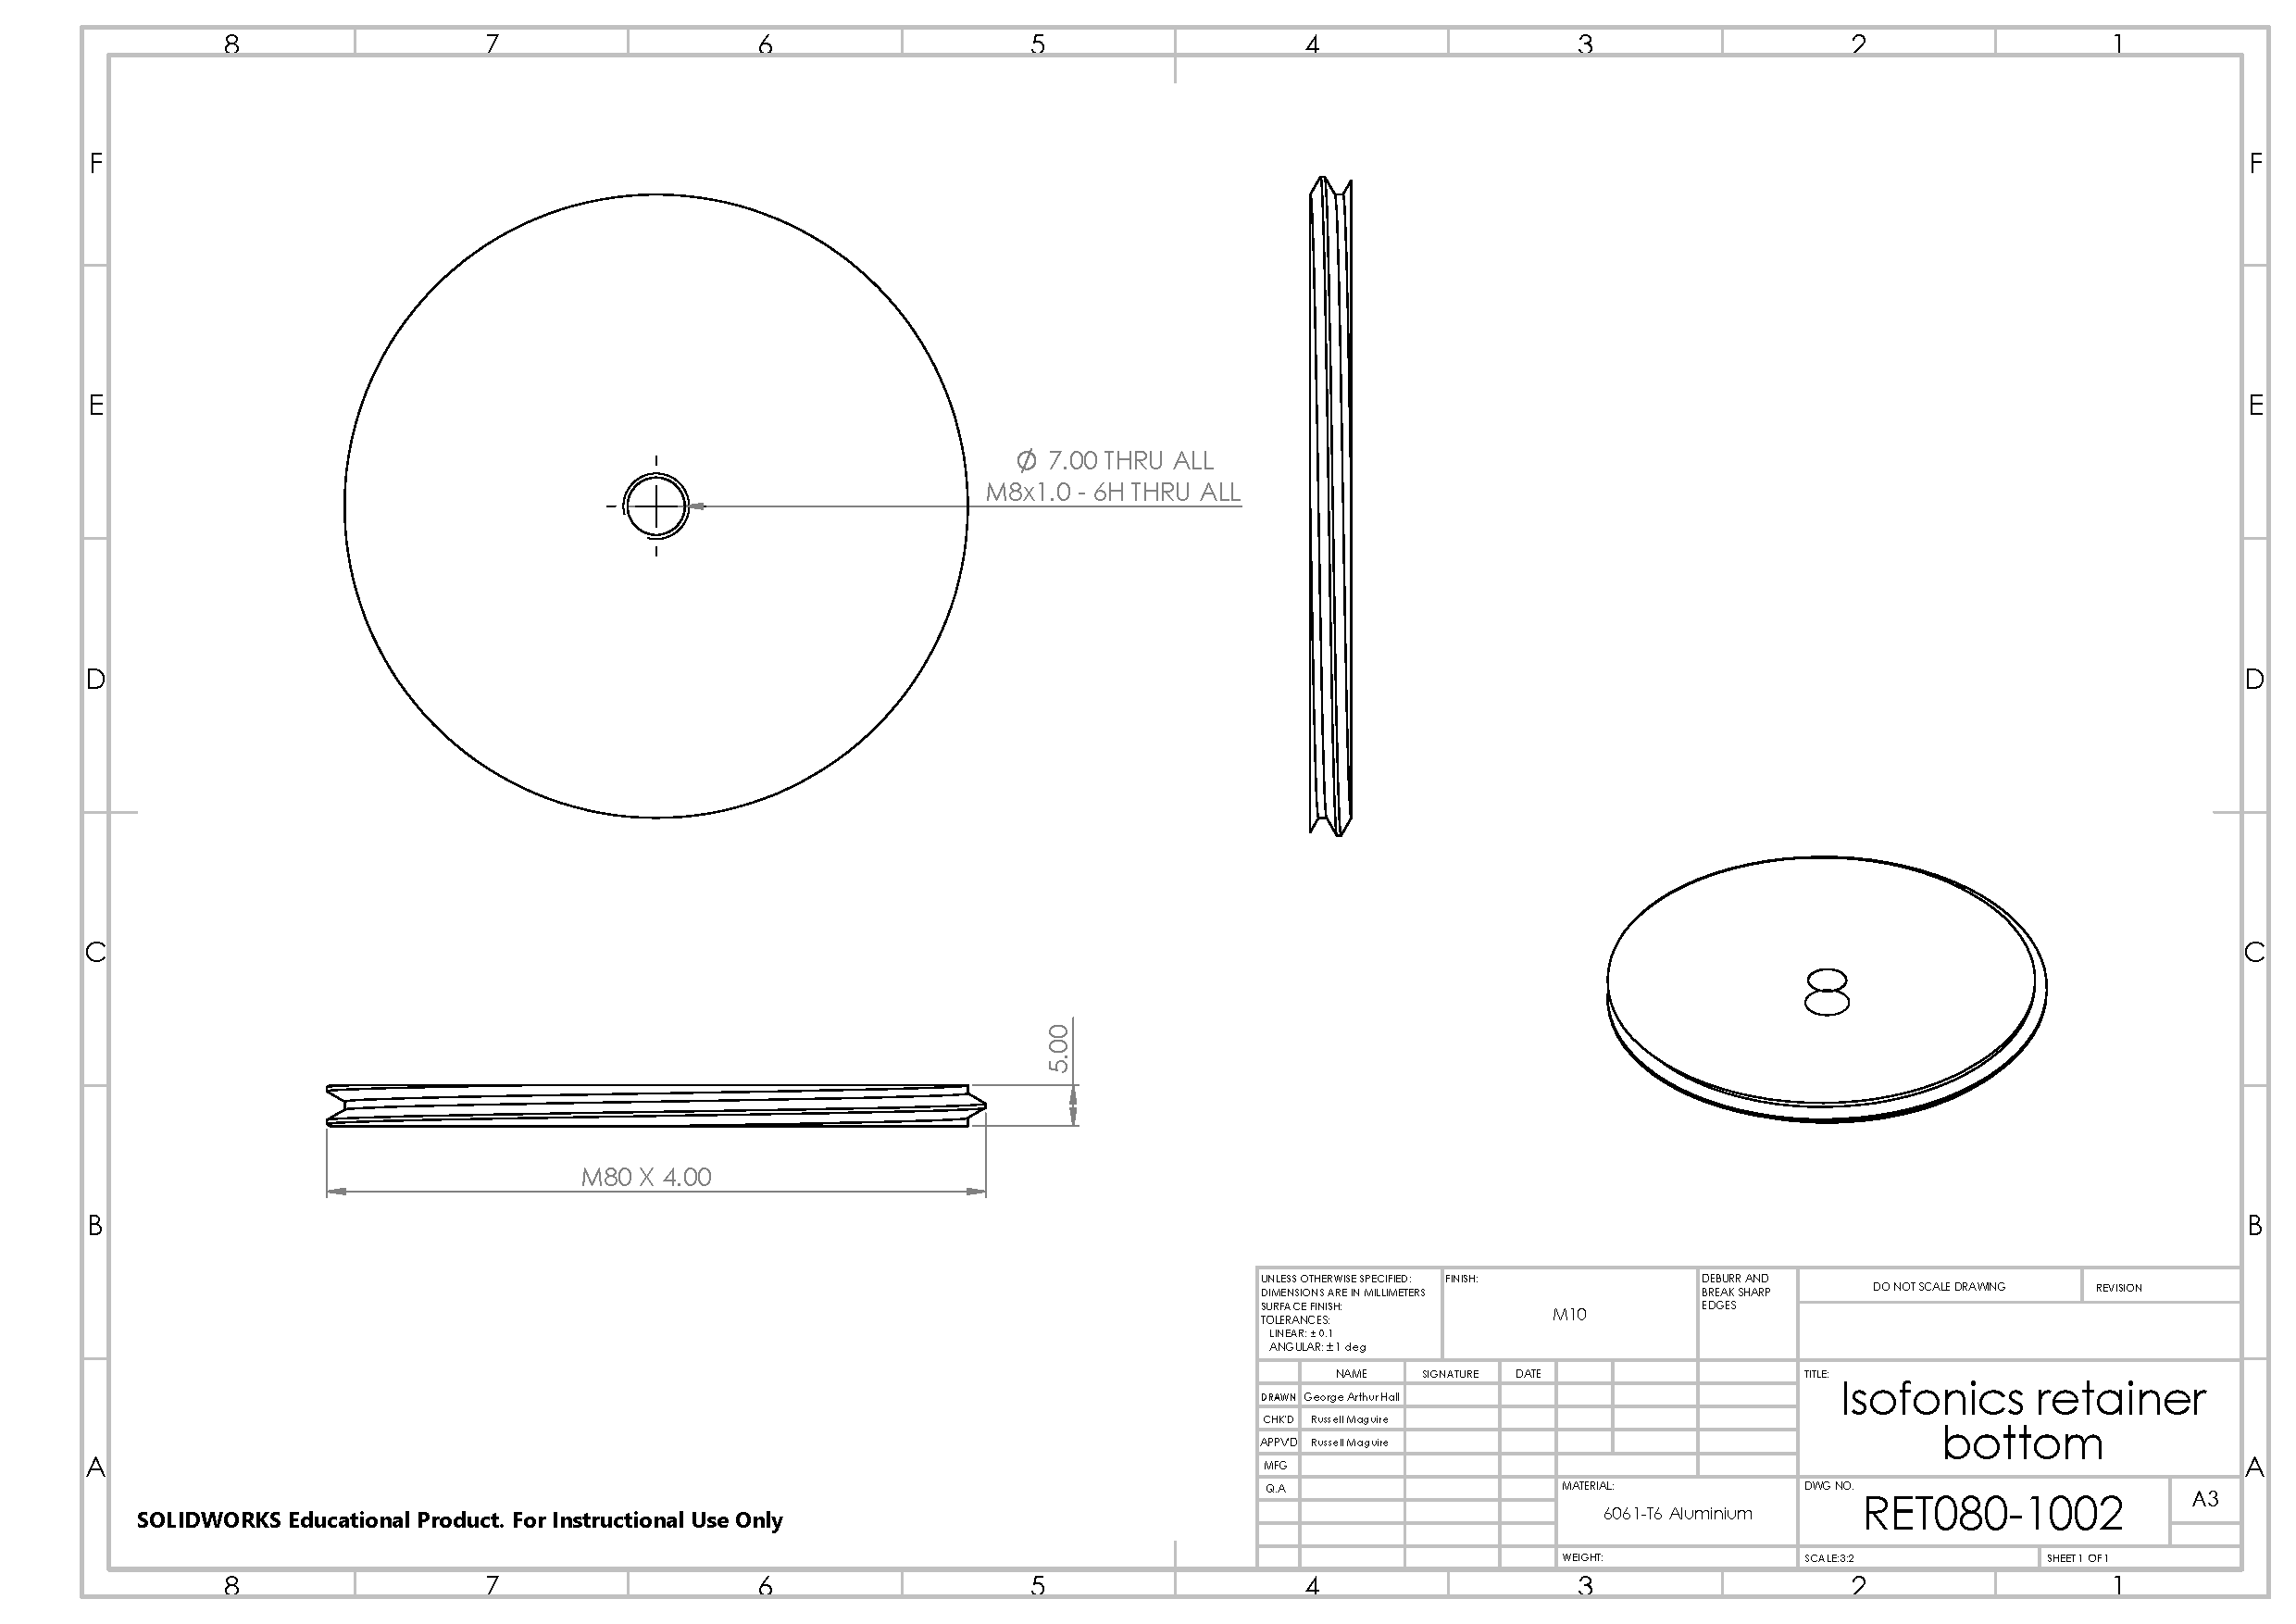
\includepdf[pages=-,fitpaper=true]{Images/Drawings/RET080-1002.PDF}
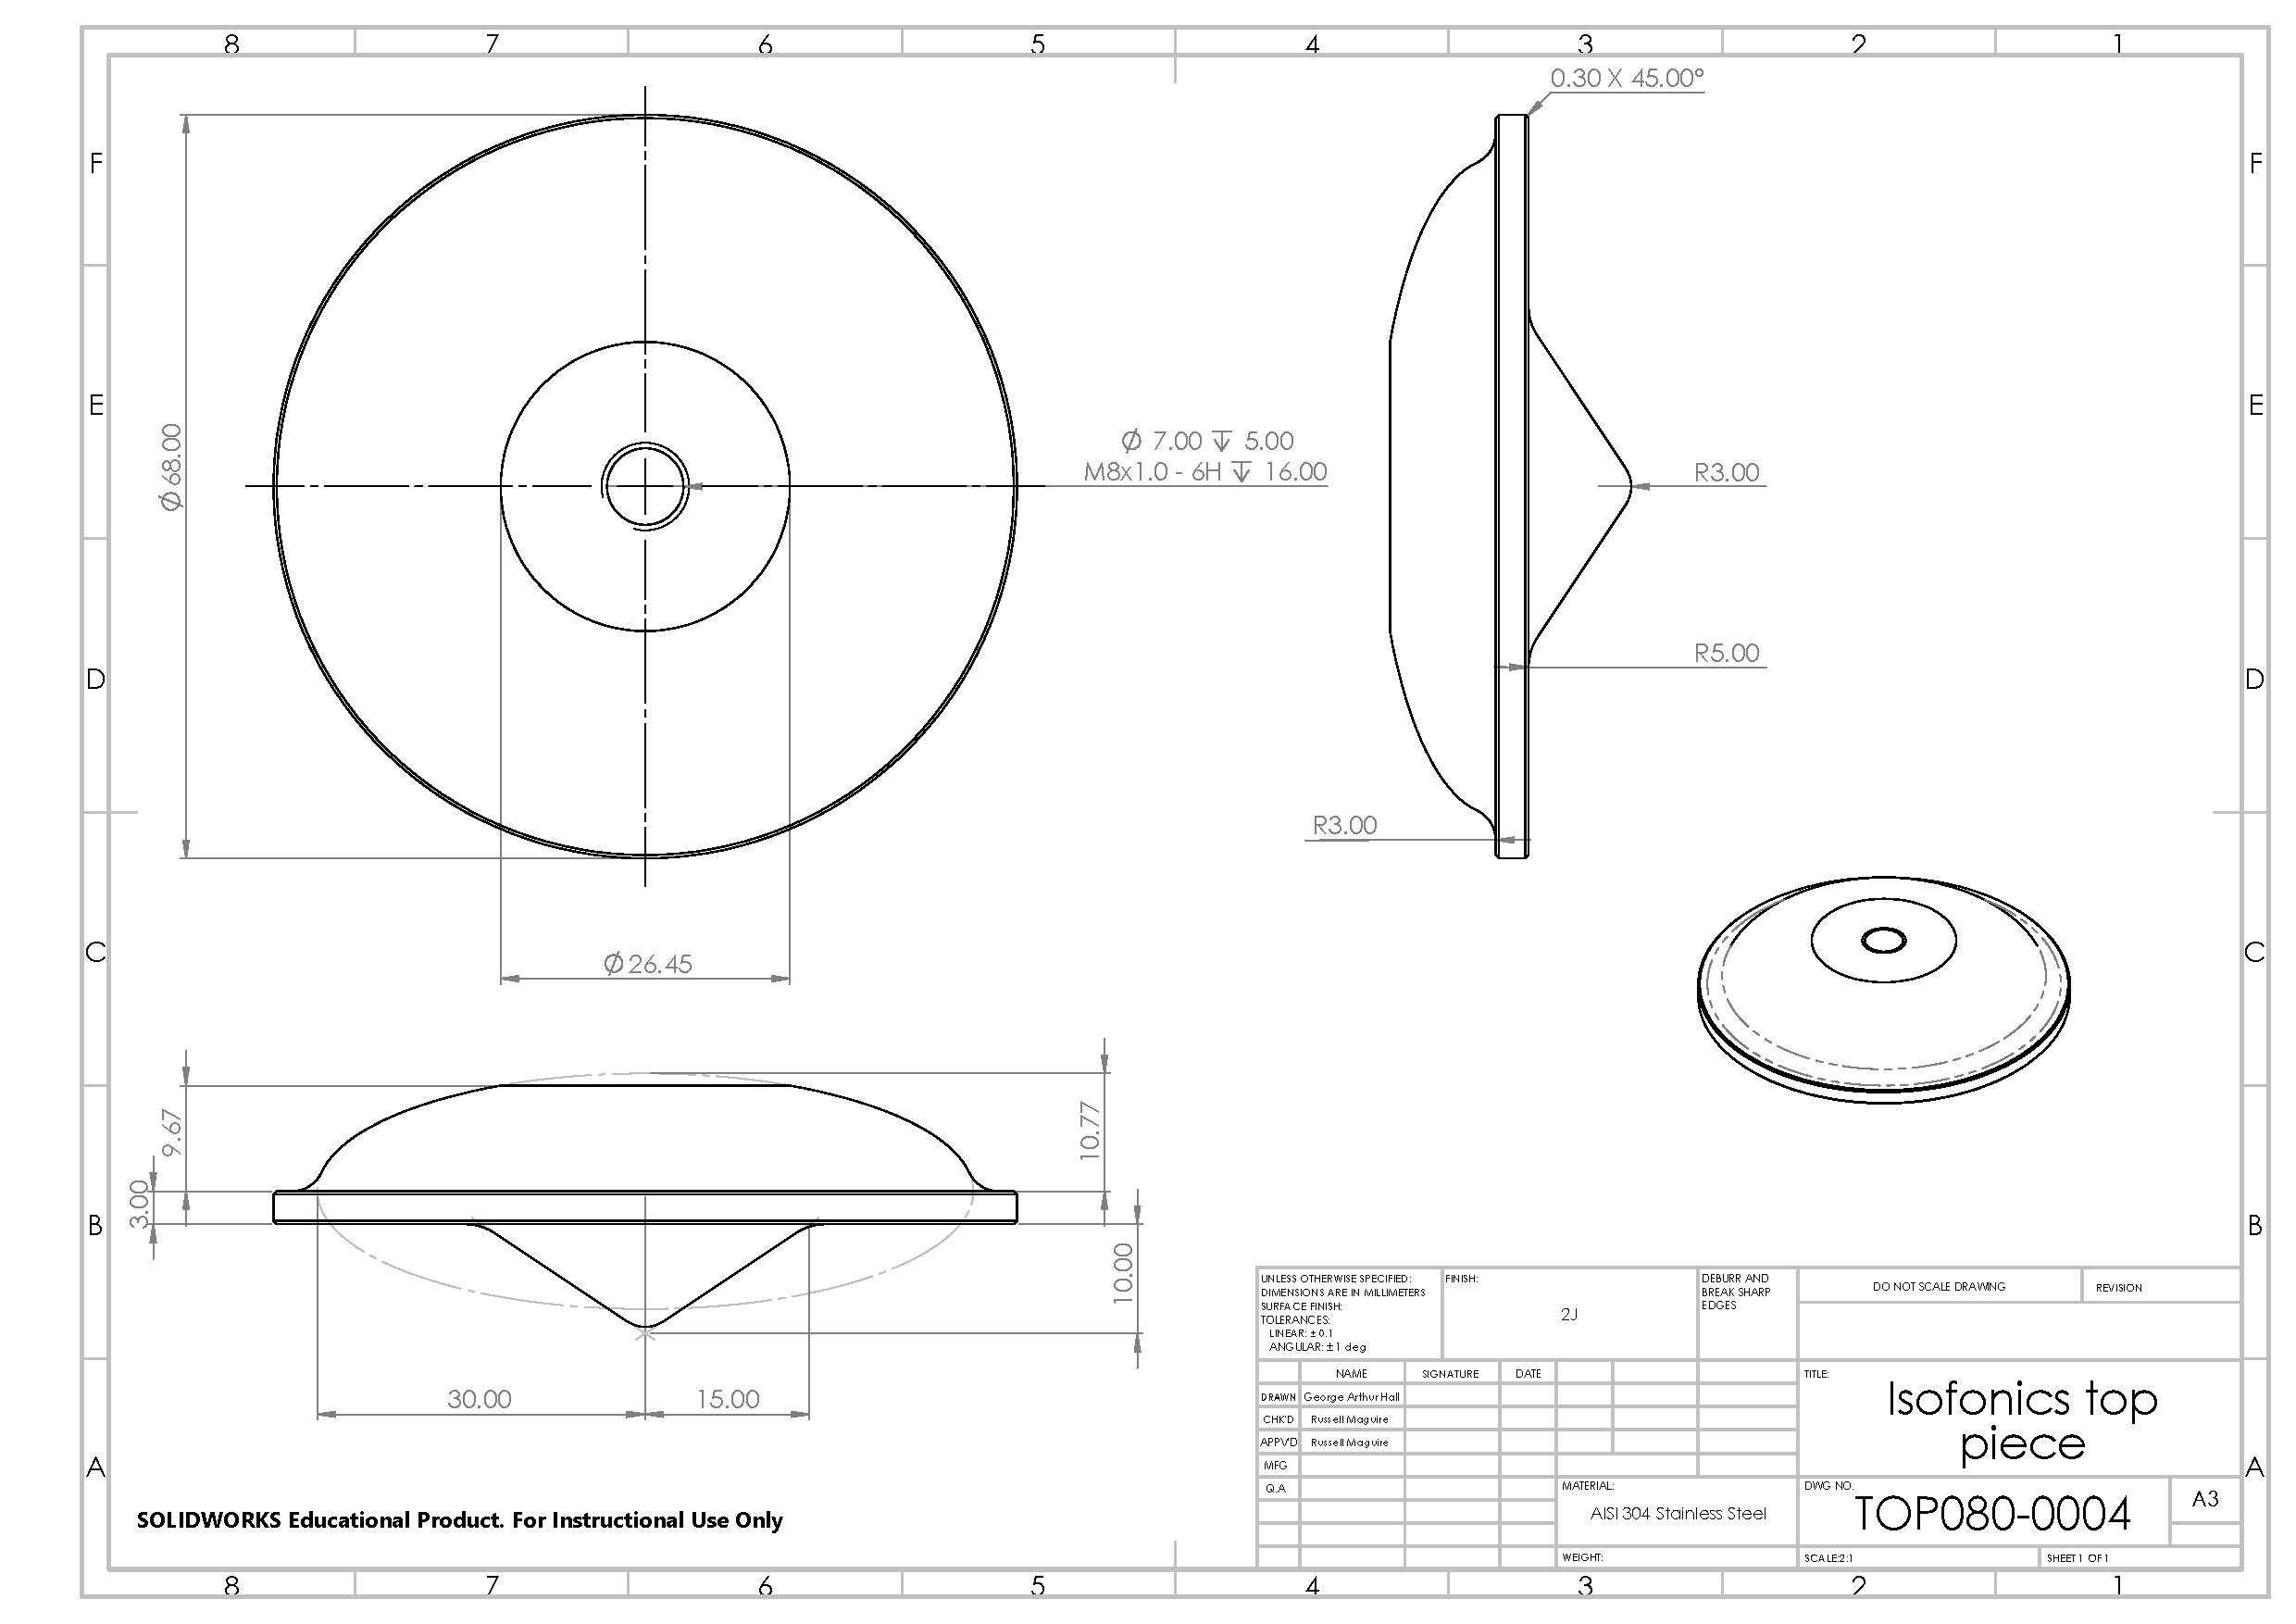
\includepdf[pages=-,fitpaper=true]{Images/Drawings/TOP080-0004.PDF}
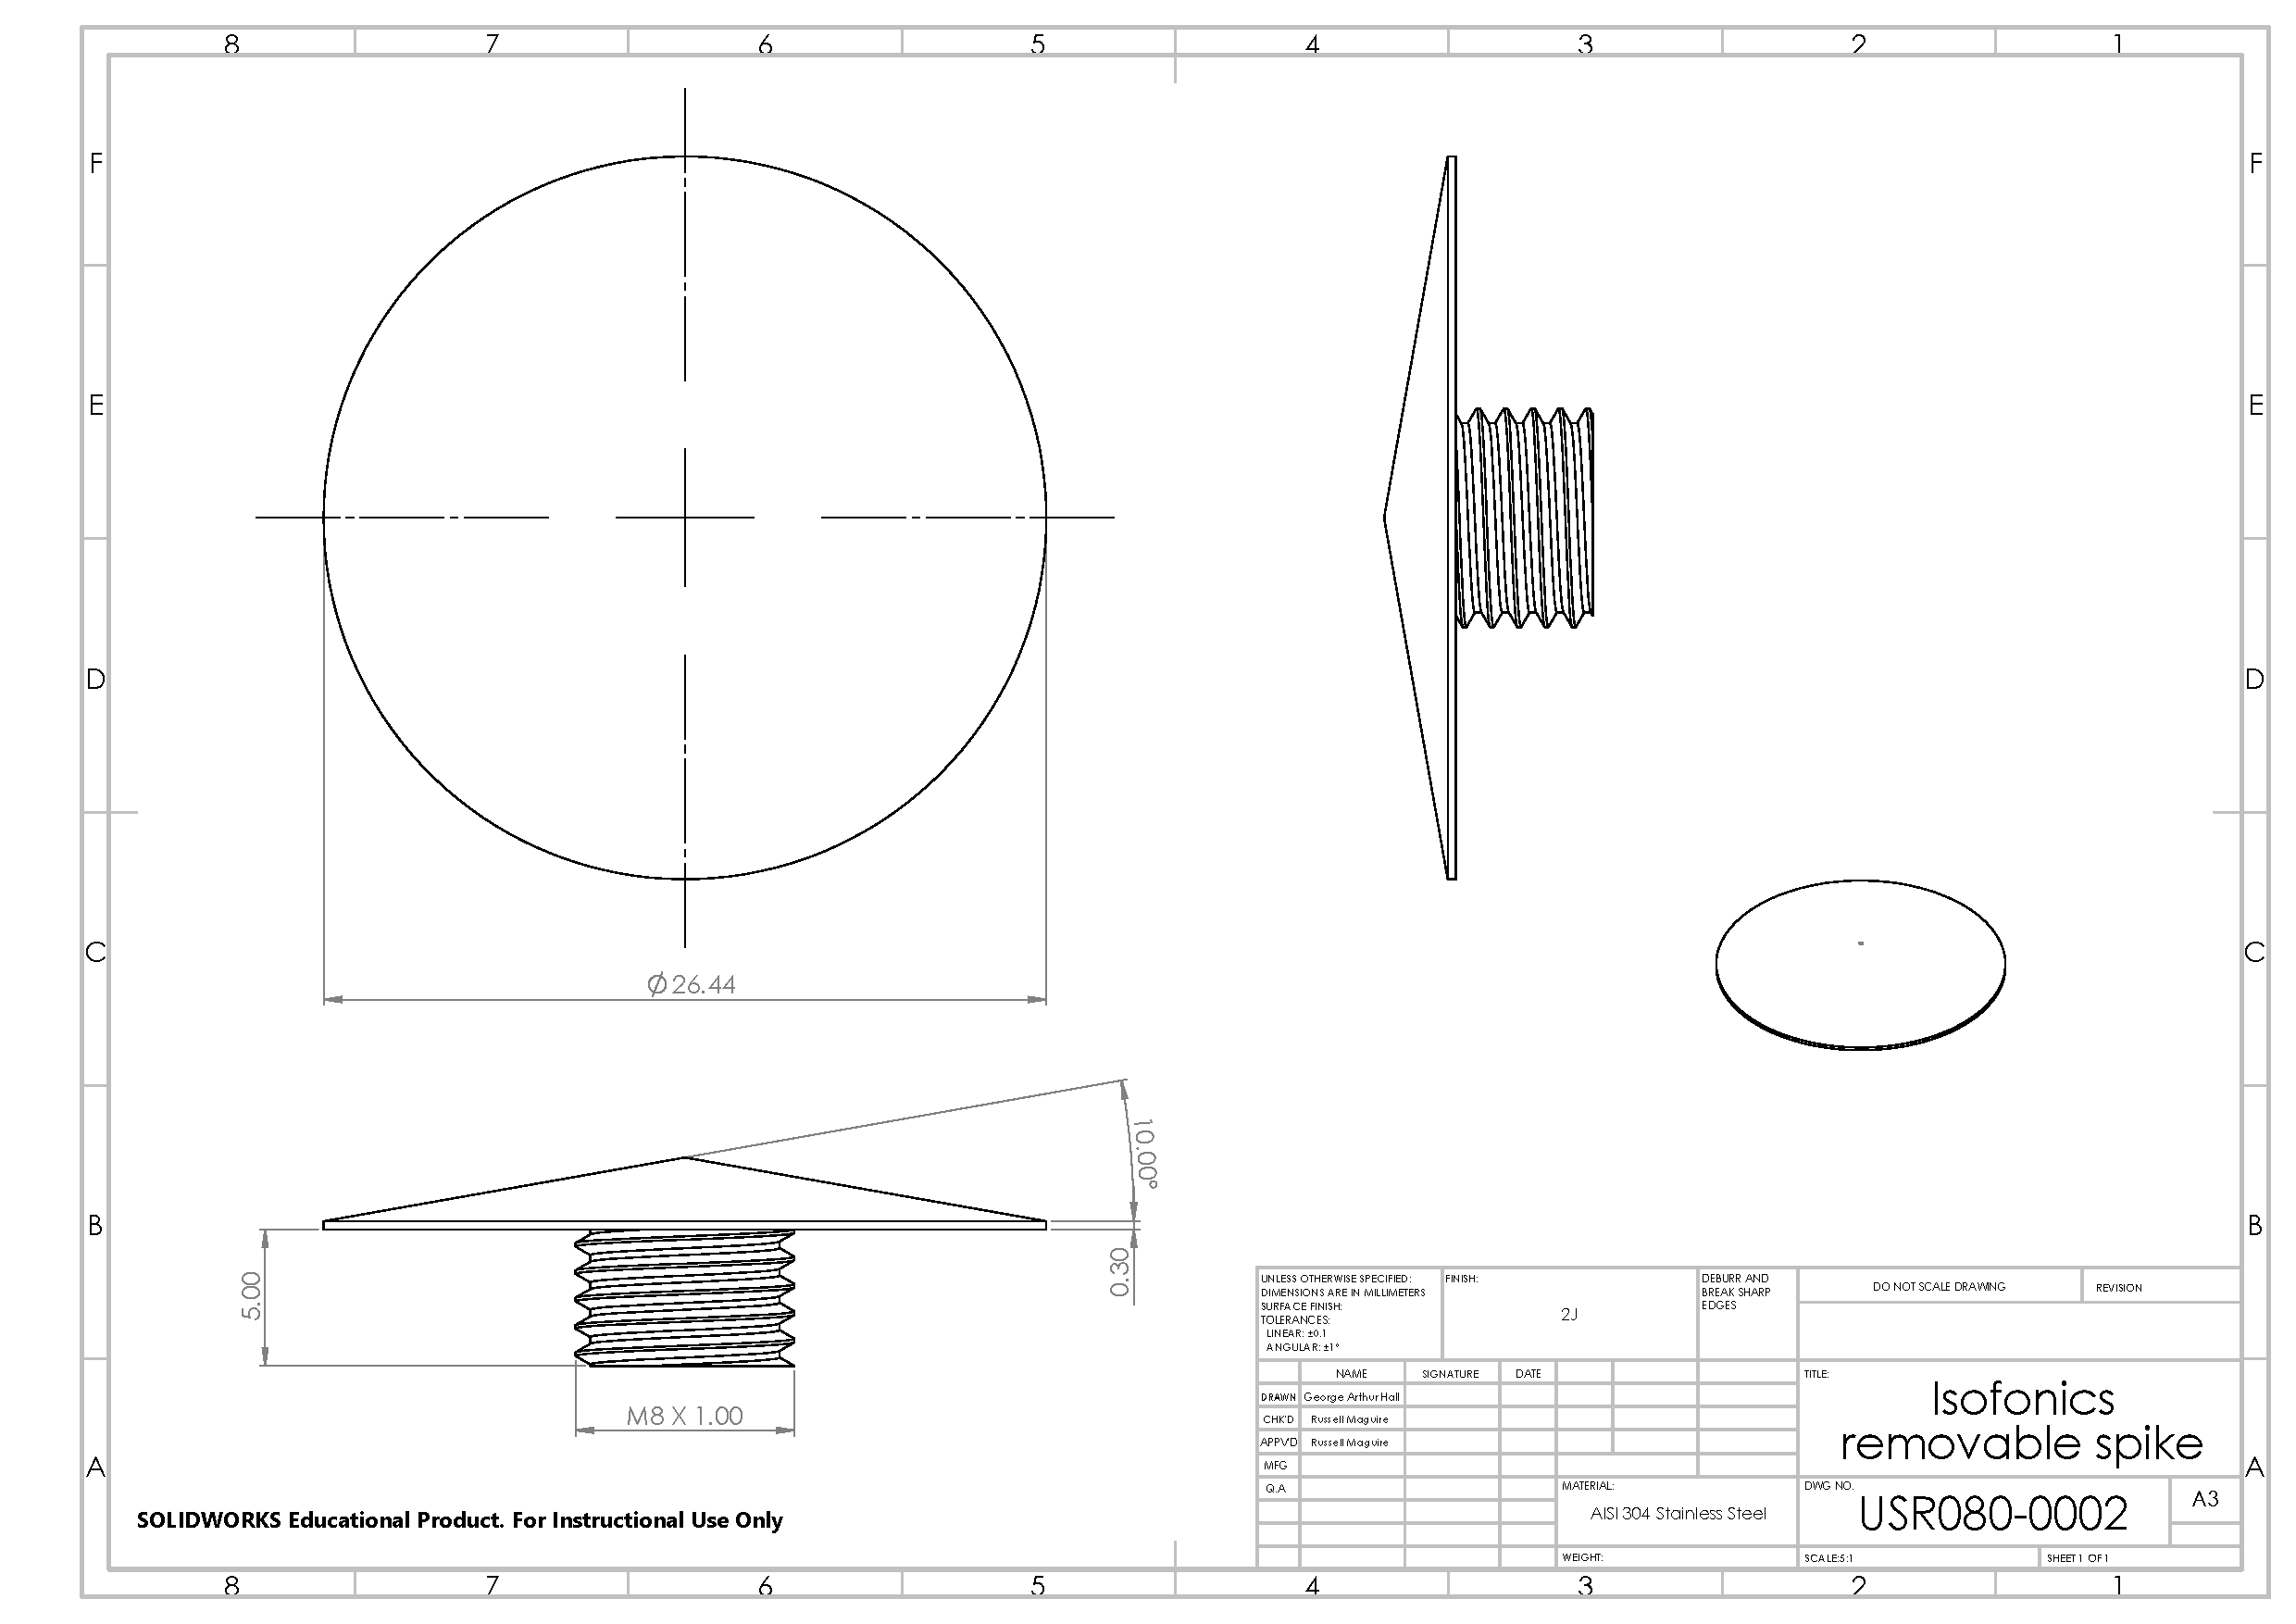
\includepdf[pages=-,fitpaper=true]{Images/Drawings/USR080-0002.PDF}
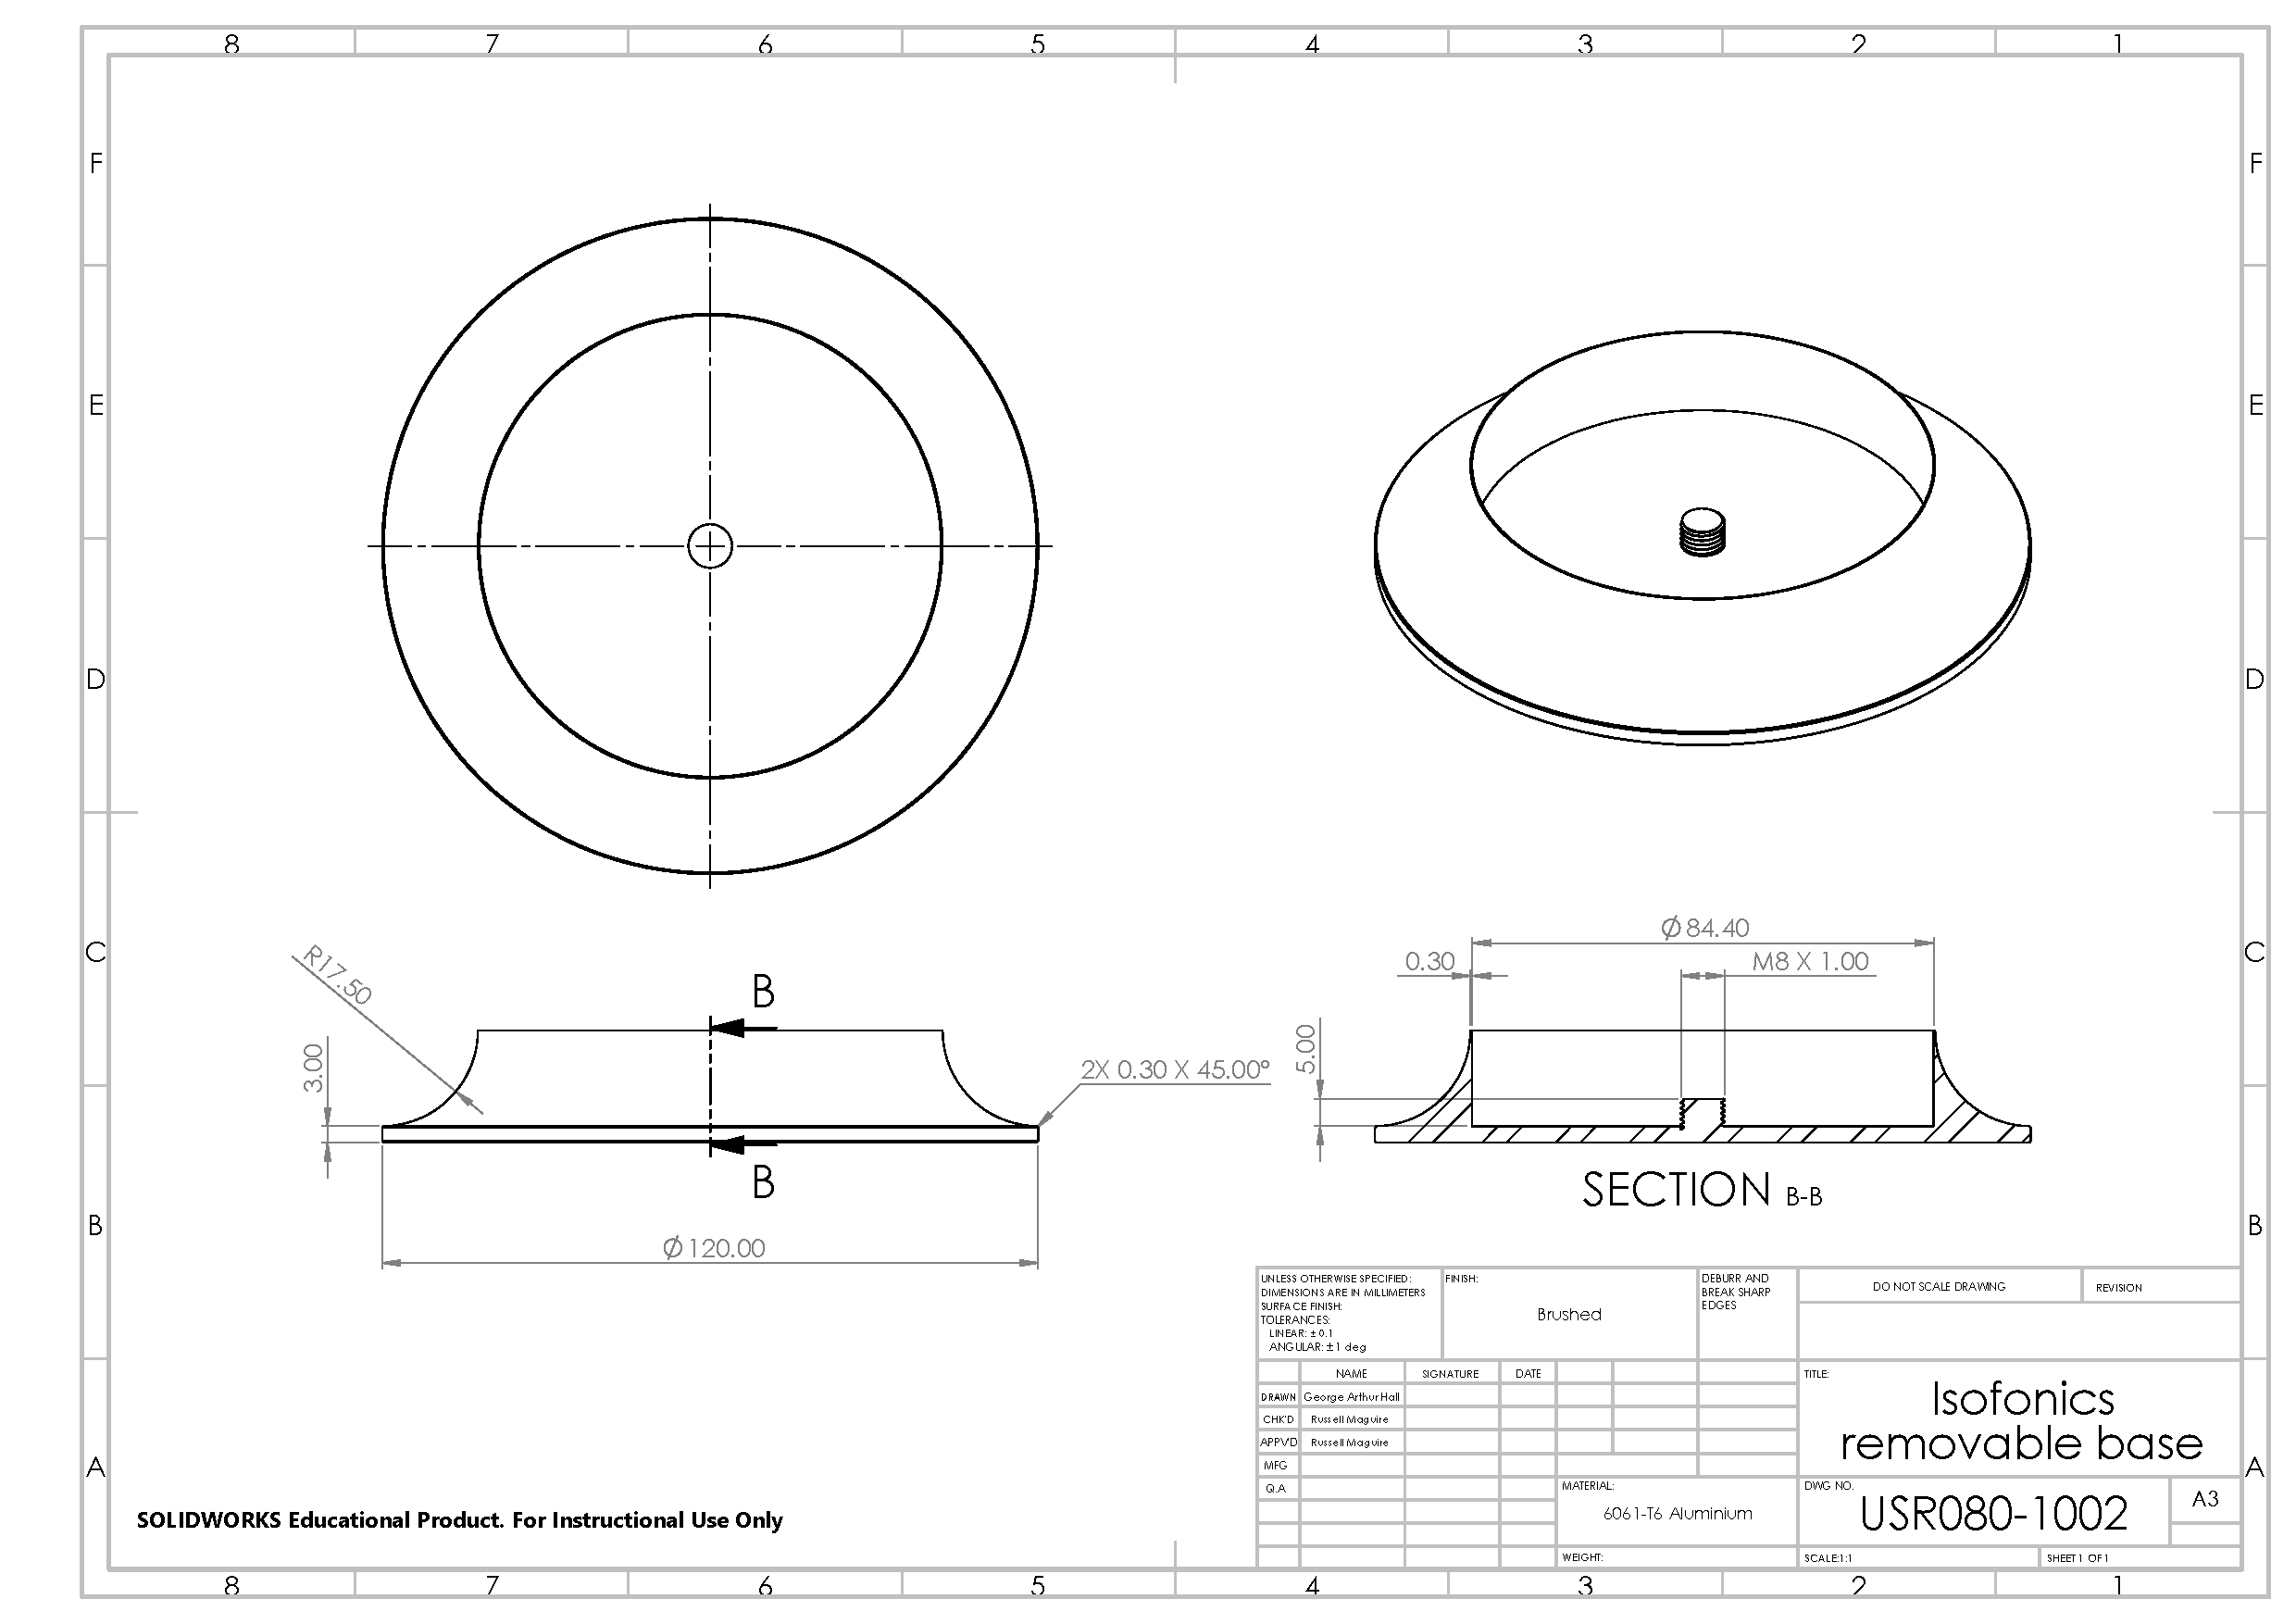
\includepdf[pages=-,fitpaper=true]{Images/Drawings/USR080-1002.PDF}

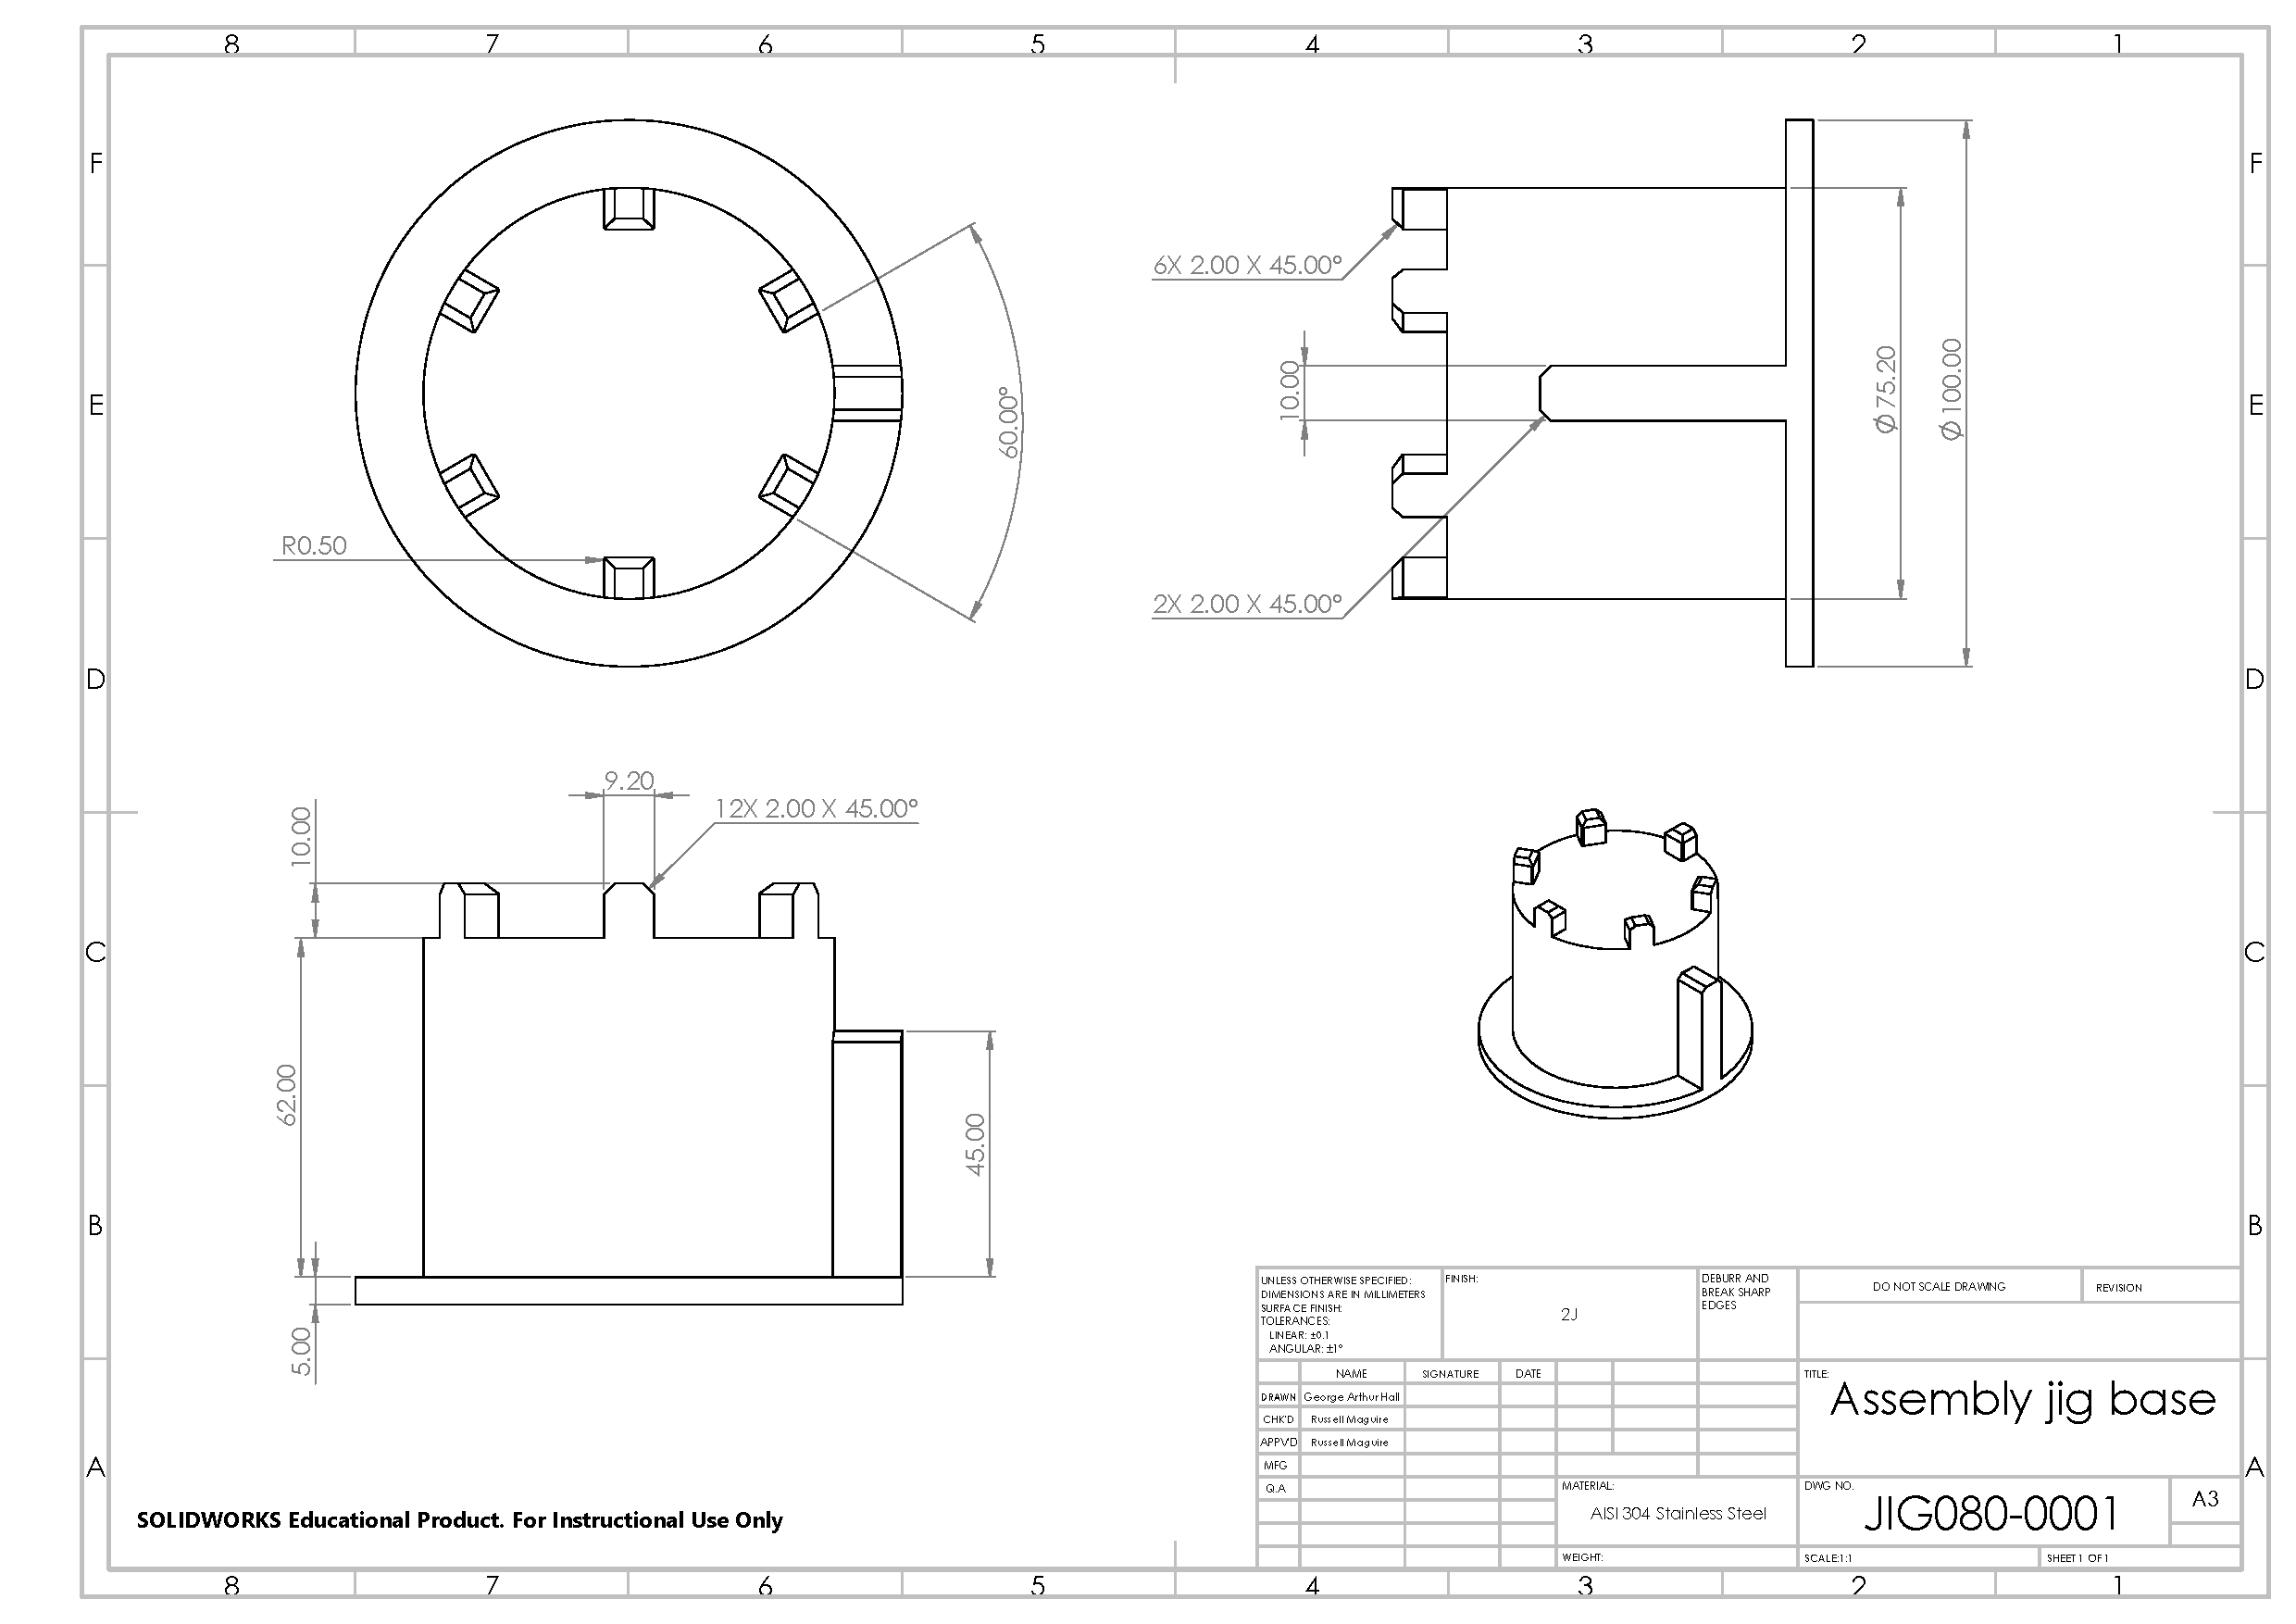
\includepdf[pages=-,fitpaper=true]{Images/jig/JIG080-0001.PDF}
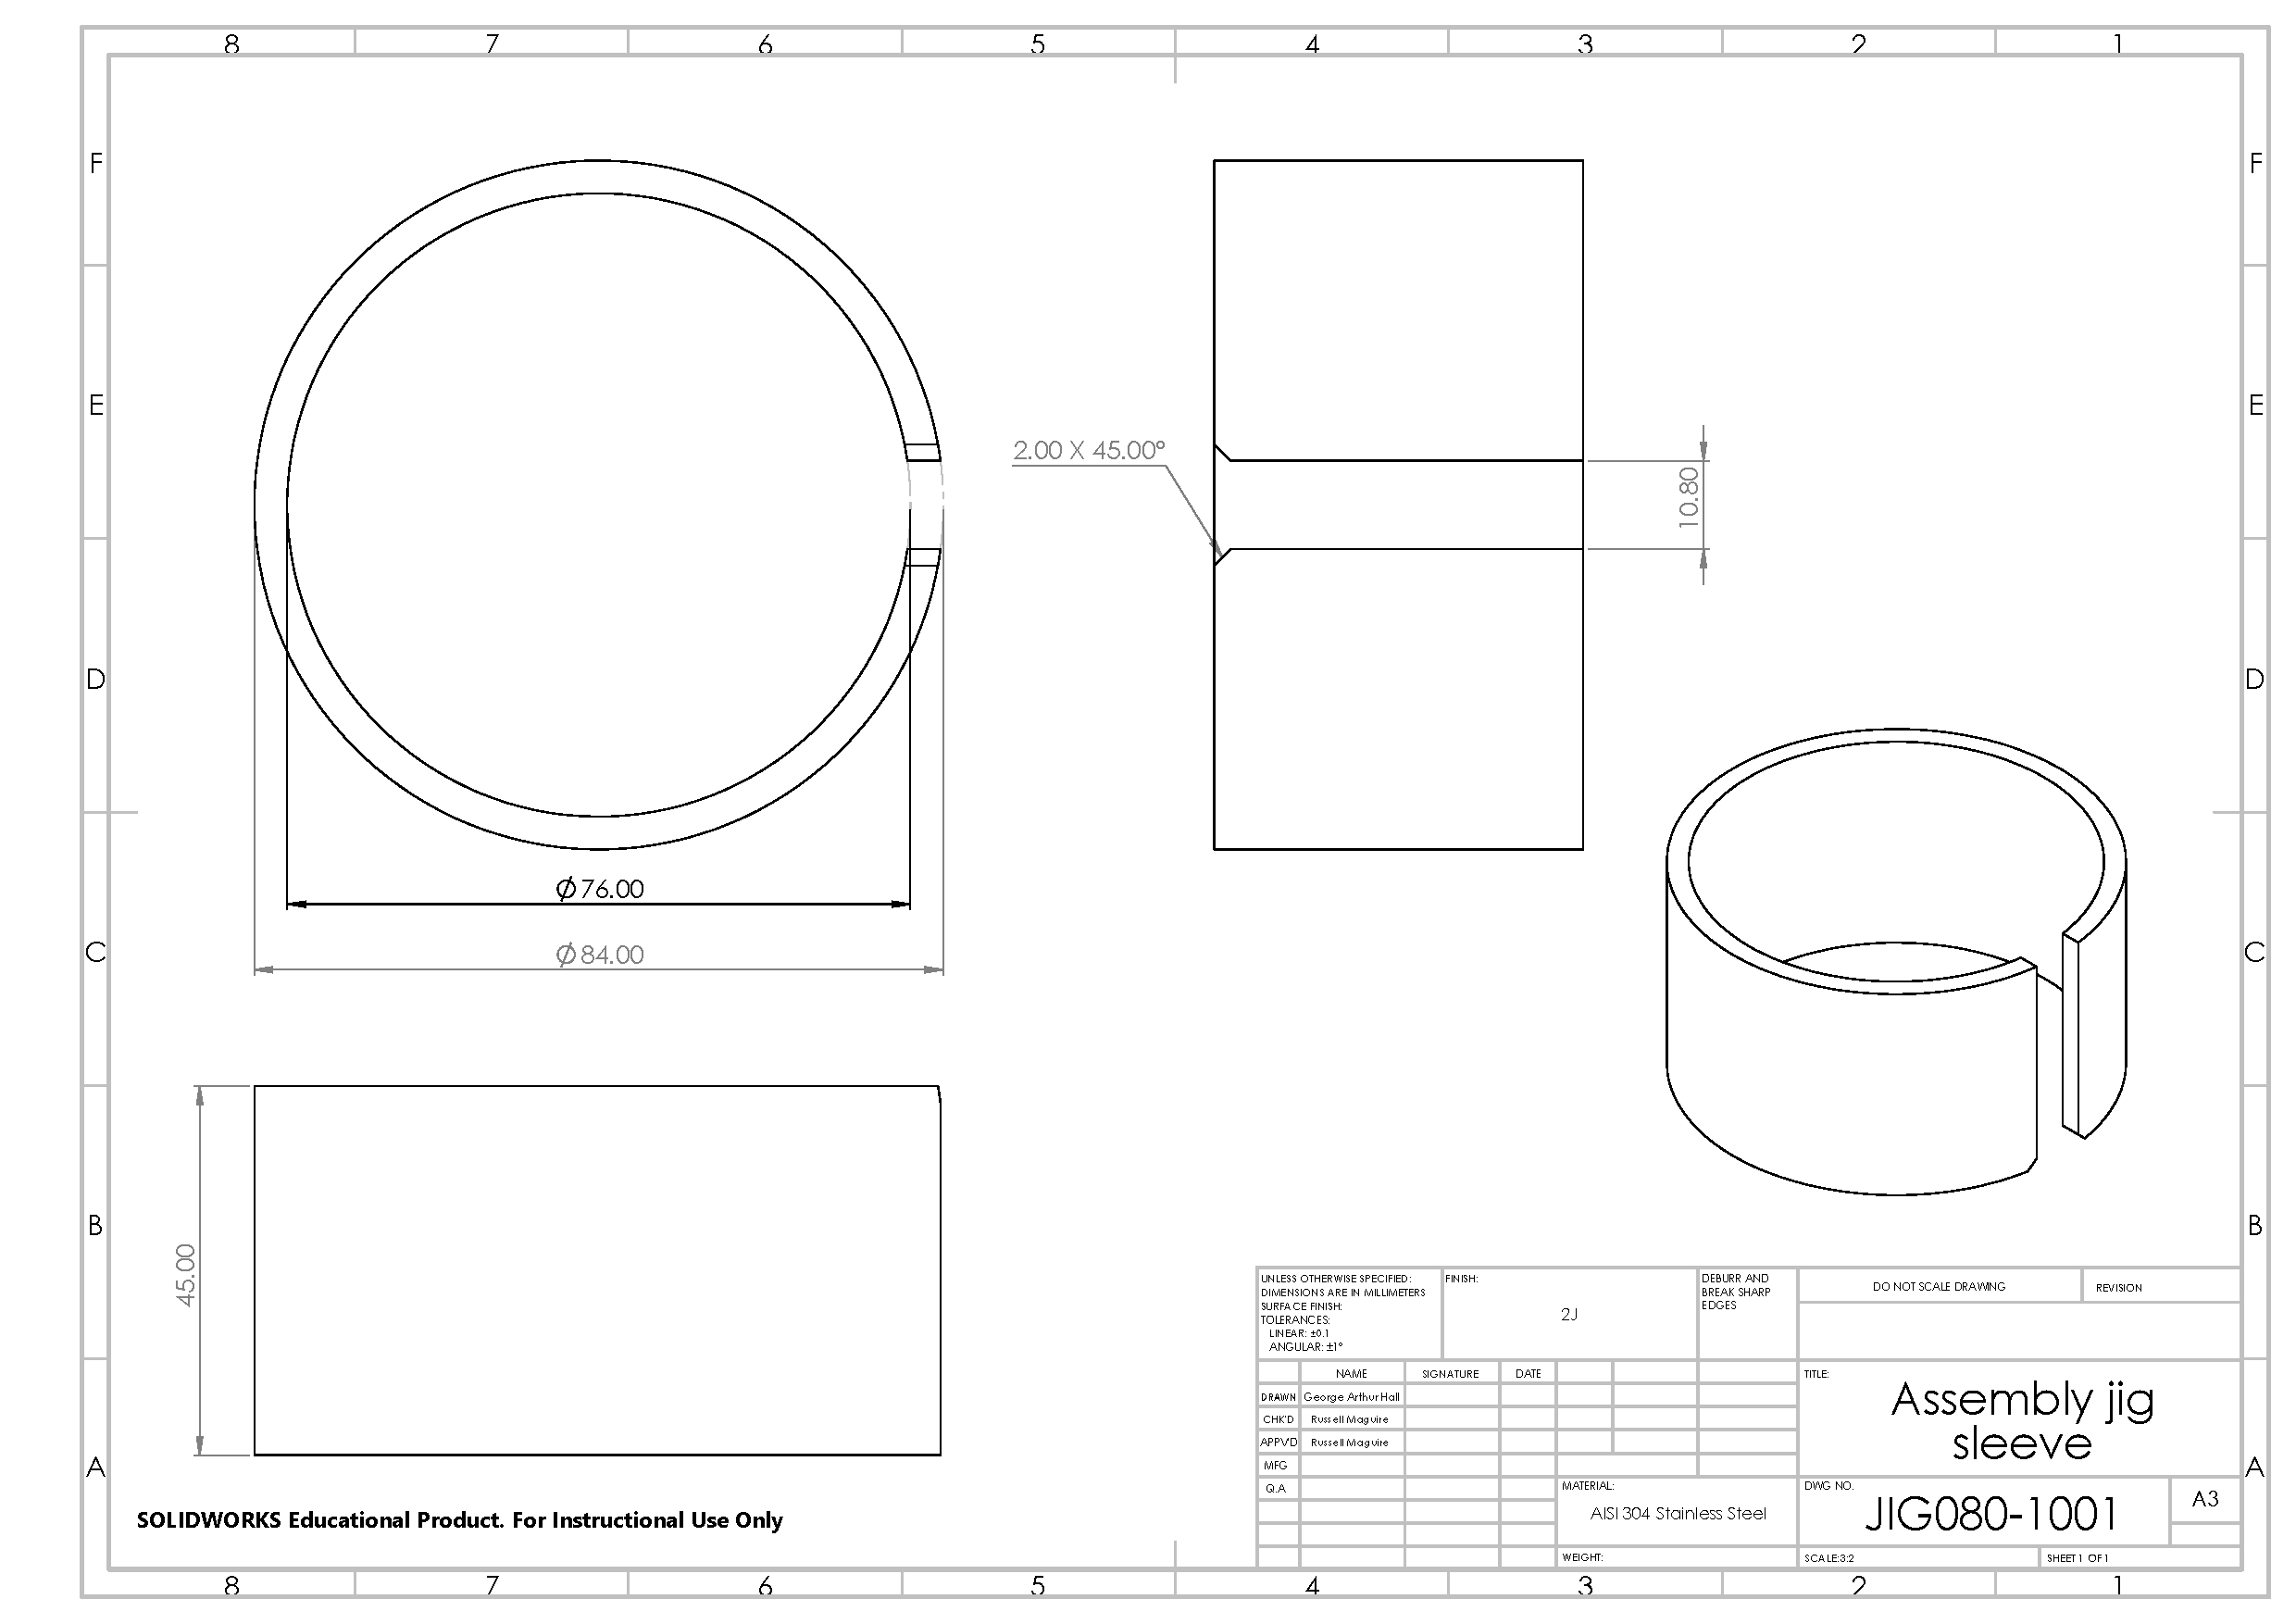
\includepdf[pages=-,fitpaper=true]{Images/jig/JIG080-1001.PDF}

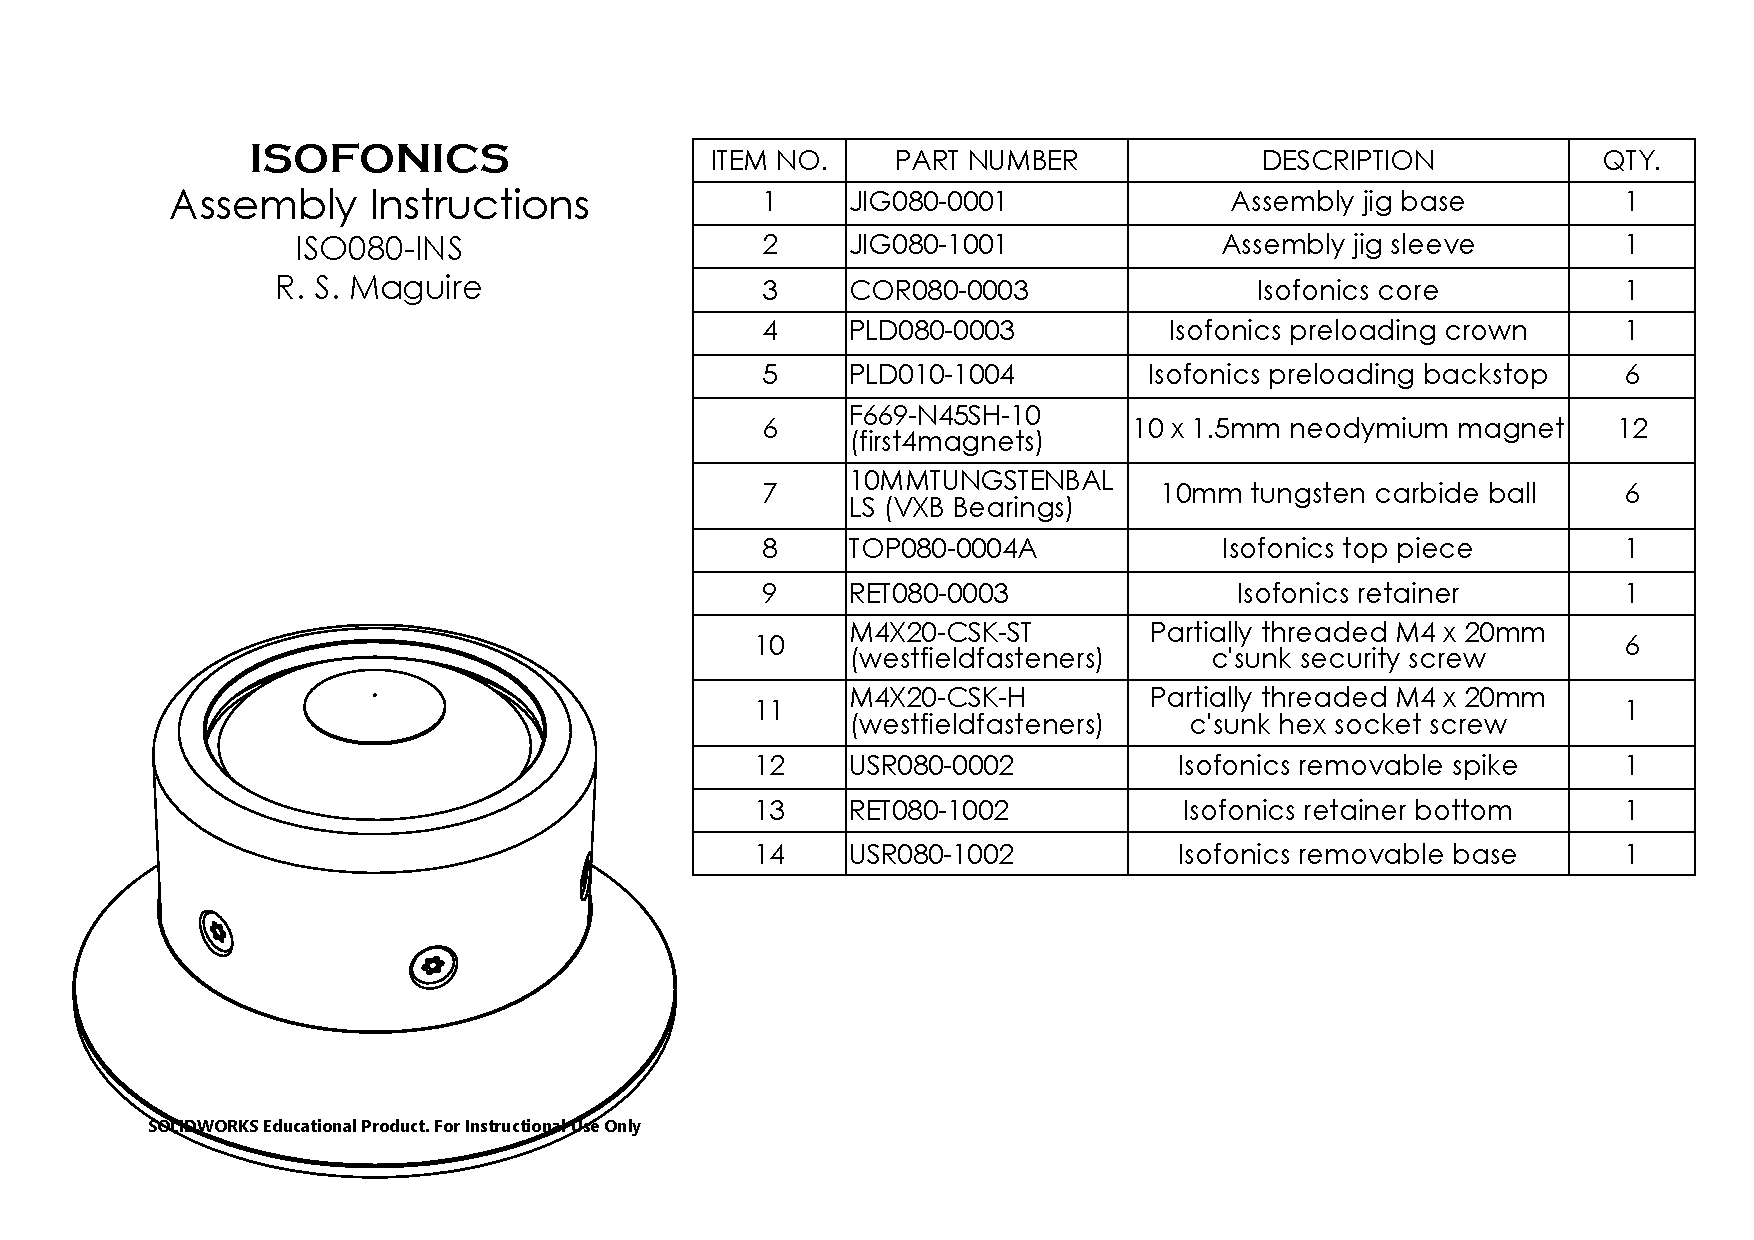
\includepdf[pages=-,fitpaper=true]{Images/jig/ISO080-INS.pdf}



\end{document}
